\documentclass[letterpaper,conference]{IEEEtran}
\usepackage[utf8]{inputenc}
\usepackage{float}
\usepackage{graphicx}
\usepackage{caption}
\usepackage{subcaption}
\usepackage{booktabs} % For formal tables
\usepackage{array}
\usepackage{multirow}
\usepackage{amssymb}
\usepackage{algorithmicx,algorithm}
\usepackage[noend]{algpseudocode}
\usepackage{tikz}
\usepackage{varwidth}
\usepackage{amsmath}
\usetikzlibrary{backgrounds}%arrows, shapes, trees, 
\usetikzlibrary{positioning}
\usetikzlibrary{shapes.geometric, arrows}

\makeatletter
\let\OldStatex\Statex
\renewcommand{\Statex}[1][3]{%
  \setlength\@tempdima{\algorithmicindent}%
  \OldStatex\hskip\dimexpr#1\@tempdima\relax}
\makeatother

% Copyright
%\setcopyright{none}
%\setcopyright{acmcopyright}
%\setcopyright{acmlicensed}
%\setcopyright{rightsretained}
%\setcopyright{usgov}
%\setcopyright{usgovmixed}
%\setcopyright{cagov}
%\setcopyright{cagovmixed}


% DOI
%\acmDOI{10.475/123_4}

% ISBN
%\acmISBN{123-4567-24-567/08/06}

%Conference
%\acmConference[MobiHoc'17]{ACM International Symposium on Mobile Ad Hoc Networking and Computing}{July 2017}{Chennai, India} 
%\acmYear{2017}
%\copyrightyear{2017}

%\acmPrice{15.00}


\begin{document}
\title{Enhancing Throughput in Cognitive Multi-Radio Networks}
%\titlenote{Produces the permission block, and
%  copyright information}
%\subtitle{Extended Abstract}
%\subtitlenote{The full version of the author's guide is available as
%  \texttt{acmart.pdf} document}

\iffalse
\author{Tanvir~Ahmed~Khan}
%\authornote{Dr.~Trovato insisted his name be first.}
\orcid{1234-5678-9012}
\affiliation{%
  \institution{Dept. of Computer Science \& Engineering\\Bangladesh University of Engineering and Technology}
  %\streetaddress{P.O. Box 1212}
  \city{Dhaka} 
  \state{Bangladesh} 
  %\postcode{43017-6221}
}
\email{takhan@cse.buet.ac.bd}

\author{A.~B.~M.~Alim~Al~Islam}
%\authornote{The secretary disavows any knowledge of this author's actions.}
\affiliation{%
  \institution{Dept. of Computer Science \& Engineering\\Bangladesh University of Engineering and Technology}
  %\streetaddress{P.O. Box 1212}
  \city{Dhaka} 
  \state{Bangladesh} 
  %\postcode{43017-6221}
}
\email{alim_razi@cse.buet.ac.bd}

% The default list of authors is too long for headers}
\renewcommand{\shortauthors}{T.~A.~Khan et al.}
\fi

\author{\IEEEauthorblockN{Tanvir~Ahmed~Khan}
\IEEEauthorblockA{Dept. of Computer Science \& Engineering\\Bangladesh University of Engineering and Technology\\
Dhaka, Bangladesh \\
  %\postcode{43017-6221}\\
Email: takhan@cse.buet.ac.bd}
\and
\IEEEauthorblockN{A.~B.~M.~Alim~Al~Islam}
\IEEEauthorblockA{Dept. of Computer Science \& Engineering\\Bangladesh University of Engineering and Technology\\
Dhaka, Bangladesh \\
  %\postcode{43017-6221}\\
Email: alim\_razi@cse.buet.ac.bd}\\}

\maketitle

\begin{abstract}
In recent years, Cognitive Radio Networks (CRNs) have been widely investigated to solve spectrum scarcity problem. However, little research efforts have been spent on incorporating multiple radios in CRNs. Existing studies propose several medium access control and routing protocols for Cognitive Multi-Radio Networks (CMRNs), however, none of them focuses on enhancing throughput in the network to the best of our knowledge. Therefore, in this paper, we propose a feedback-based multi-radio exploitation approach for CRNs where information obtained from lower layer (Physical layer) is incorporated in the process of decision making in an upper layer (Data Link layer) to enhance network throughput. We implement our proposed approach in \texttt{ns-3} to measure different performance metrics including throughput, delay, and drop ratio. We compare the performance against that of existing approaches for CMRNs. Simulation results suggest that our proposed feedback-based approach always achieves substantially improved network throughput compared to existing approaches, in parallel to achieving improved delay and drop-ratio in most of the cases.\vspace*{-0.5cm}
\end{abstract}

%
% The code below should be generated by the tool at
% http://dl.acm.org/ccs.cfm
% Please copy and paste the code instead of the example below. 
%
\iffalse
\begin{CCSXML}
<ccs2012>
    <concept>
        <concept_id>10003033.10003039.10003056</concept_id>
        <concept_desc>Networks~Cross-layer protocols</concept_desc>
        <concept_significance>500</concept_significance>
    </concept>
    <concept>
        <concept_id>10003033.10003079</concept_id>
        <concept_desc>Networks~Network performance evaluation</concept_desc>
        <concept_significance>500</concept_significance>
    </concept>
</ccs2012>
\end{CCSXML}

\ccsdesc[500]{Networks~Cross-layer protocols}
\ccsdesc[500]{Networks~Network performance evaluation}

% We no longer use \terms command
%\terms{Theory}

\keywords{Cognitive radio networks, cross-layer protocols}
\fi

\IEEEpeerreviewmaketitle

%\input{samplebody-conf}

\section{Introduction}
% What is the problem?
The famous spectrum scarcity problem along with significant spectrum under-utilization in traditional spectrum management has lead towards the notion of dynamic spectrum access~\cite{akyildiz2006next} through cognitive radios. A \textit{cognitive radio} monitors its operational electromagnetic environment to dynamically adjust its operating parameters.%~\cite{Mitola}
 Thus, a cognitive radio is capable of accessing a temporal free spectrum. Cognitive Radio Networks (CRNs) exploit  cognitive radios through comprising two types of users. The first type refers to \textit{primary users} (PUs), who possess licenses to operate in the spectrum bands. The second type refers to \textit{secondary users} (SUs), who are unlicensed and employ cognitive radios to opportunistically access instantaneous spectrum holes.

% Why is it interesting and important?
%The importance of our study lies on the fact that almost all the modern mobile devices contain multiple radios.

On the other hand, classical wireless networks frequently adopt the notion of deploying users with multiple radios~\cite{bahl2004reconsidering}. Such deployment of multiple radios improves capacity of the networks~\cite{bahl2004reconsidering}, enhances loss resilience~\cite{miu2005improving}, and enables heterogeneous wireless access~\cite{song2012performance}. However, this augmentation also demands modified transport, routing, and link-layer protocols~\cite{kyasanur2006routing, chatterjee2013low}. Nonetheless, as such deployment of multiple radios in wireless nodes is known to improve the performance of a user and  deployment of cognitive radios also aims to improve the performance of secondary users through spectrum utilization, it is intuitive that simultaneous utilization of both these techniques, i.e., Cognitive Multi-Radio Networks (CMRNs), will result in significantly improved network performance. Therefore, the notion of exploiting multiple radios in CRNs to supplement the dynamic spectrum access has been proposed in the contemporary literature. Existing studies in this regard present that such multi-radio deployment in CRNs improves delay up to a certain point, however, throughput gets degraded with an increase in the number of radios per secondary user~\cite{khan2015towards}. Therefore, the main motivation behind this study is to examine how to improve network throughput while equipping secondary users with multiple radios.

% Why is it hard? (E.g., why do naive approaches fail?)
%The main challenge of improving total network throughput in CMRNs lies on the silent features of the architecture of CRNs. In CRNs, nodes generally have limited spectrum knowledge covering only its own neighborhood. Thus, the knowledge is conventionally gathered in a distributed manner. Therefore, graph-based and MILP optimization-based solutions~\cite{hoang2008downlink,ahmed2014channel} for improving throughput can not be directly incorporated due to their nature of performing centralized computations.

% Why hasn't it been solved before? (Or, what's wrong with previous proposed solutions? How does mine differ?)
Most of the existing studies~\cite{ahmadi2012distributed, zhong2014capacity, li2014deterministic, khan2015towards} on CMRNs fail to solve our research problem, as they overlook the effect of utilizing multiple radios on different performance metrics. Besides, several studies~\cite{de2012survey, feng2009joint, zhong2014capacity, li2014deterministic} usually integrate MAC and routing protocols for the multi-radio network architectures and solve the channel assignment problem for multi-channel scenario. While assigning multiple channels among multiple radios, the existing studies either randomly select the channels~\cite{khan2015towards} or only rank the channels~\cite{zhong2014capacity}. Due to these reasons, to the best of our knowledge, no existing study provides a viable solution for enhancing throughput in CMRNs. Moreover, the relation between two different performance metrics (throughput and delay) may be opposing in nature~\cite{gamal2004throughput} and improving one of them may result in degradation of the another. Consequently, a trade-off between these two metrics demands a special attention in CMRNs in road to improving throughput.

% What are the key components of my approach and results? Also include any specific limitations.
To this end, in this paper, we propose a specialized mechanism of incorporating feedback obtained from radio transmission environment in the process of decision making in Data Link layer to enhance network throughput. Here, to obtain lower layer feedback, we keep different packet counters for radios as well as channels in each secondary user. Using values of these counters, we rank all available radios and channels of a secondary user. Subsequently, based on the ranking, we make packet queuing decisions and channel switching decisions from the Data Link layer while retaining a stochastic flavor. We implement our proposed feedback-based approach in \texttt{ns-3} to evaluate its performance in terms of throughput along with delay and drop ratio. Simulation results confirm that our proposed approach can achieve significant improvement in terms of all the performance metrics.

% Summary of Contributions
%Then have a final paragraph or subsection: "Summary of Contributions". It should list the major contributions in bullet form, mentioning in which sections they can be found. This material doubles as an outline of the rest of the paper, saving space and eliminating redundancy.

Based on our study, in this paper, we make the following set of contributions:

\begin{itemize}
\item We propose a feedback-based multi-radio exploitation approach, along with several variants, to solve the throughput degradation problem in CMRNs.
\item We implement the proposed approach and its variants in \texttt{ns-3} to demonstrate efficacy of their radio and channel selection policies with an increasing number of radios.
\item We compare performance of our proposed approach against that of existing approaches in the literature. Comparative results reveal significant improvement over existing approaches through using our proposed approach.
\end{itemize}

\section{Related Work}

Existing studies on CMRNs mainly investigate how to incorporate multiple radios for dynamic spectrum sharing scenario. These studies mainly propose medium access control protocols~\cite{cormio2009survey, de2012survey}, routing protocols~\cite{zhu2008stod, feng2009joint}, and channel assignment techniques~\cite{ahmadi2012distributed, zhong2014capacity} for CMRNs. For example, Zhu et al., present a spectrum-tree based on-demand routing protocol that considers multi-radio nodes~\cite{zhu2008stod}. Such nodes belong to multiple spectrum-trees and are called overlapping nodes. As these nodes simultaneously work in different spectrum-trees, they can be used for inter-spectrum routing. The study shows that the proposed approach significantly reduces average end-to-end delay.  Besides, Feng et al., propose a novel spectrum handoff scheduling approach for multi-hop CMRNs~\cite{feng2009joint}. This study presents a routing protocol with the help of aging-based priority assignment to only minimize latency. Thus, none of these approaches addresses the problem of overcoming throughput degradation problem in CMRNs.

Ahmadi et al., present one of the earliest CRN studies involving multiple radios, which considers two sender radios for each secondary user~\cite{ahmadi2012distributed}. This study strives to solve channel assignment problem for the scenario. However, as there is only one receiver radio for each user in the proposed network model and channels are assigned to the receiver radio, the corresponding channel assignment problem becomes close to the single-radio channel assignment problem. This is because, as in single-radio scenario, only one channel needs to be assigned for each receiver node and the node can not exploit multiple available channels while receiving packets. Further, the study always uses a fixed number of transmitter radios (two) and do not investigate performance of the network for varying numbers of radios.

Another CMRN study~\cite{zhong2014capacity} by Zhong et al., aims to solve the channel assignment problem for CMRNs. Here, their proposed channel assignment approach assigns multiple channels among multiple radios available for secondary users. Despite ranking channels, while assigning them among radios, the approach does not consider the state of those radios. Besides, the paper does not provide any analysis on throughput with an increase in the number of radios.

The analysis of any performance metric based on an increase in the number of radios in CRNs is first presented in the study~\cite{li2014deterministic} by Li et al., to the best of our knowledge. The study presents a rendezvous channel establishment approach for CMRNs. It shows that the maximum time to rendezvous reduces with an increase in the number of radios used in CRNs. However, the study does not provide any solution on how these radios will be used for data transmission and its subsequent effect on performance metrics such as throughput and delay.

Later, Khan et al.,~\cite{khan2015towards} propose another CMRN architecture where each secondary user employs multiple radios for data transmission. The study shows that per packet average end-to-end delay gets improved at the cost of throughput degradation with an increase in the number of radios. This study does the radio-channel assignment in a random manner and does not avoid inter-user channel interface. Thus, this study fails to improve throughput with an increase in the number of radios.

In summary, none of the existing studies focuses on enhancing throughput in CMRNs. Therefore, we attempt to propose a new channel assignment approach to enhance throughput in CMRNs in this paper. Before presenting the approach, we first elaborate our system model and problem formulation.

\section{System Model and Problem Definition}
\label{sec:systemModel}

We consider a cognitive radio network (as described in Figure~\ref{fig:systemmodel}) having $n$ primary users and $m$ secondary users in our analysis. For the sake of simplicity, we assume that $n$ primary users use $n$ distinct spectrum channels. Primary users randomly become active and inactive in their respective channel following a Poisson process~\cite{Ross}. Dedicated single PU for a single channel can actually model multiple PUs per channel. Also, when PU becomes active, SUs' transmission is held back instantly. Therefore, PUs do not refrain from using their dedicated channel. Besides, each of the $m$ secondary users has at least $2$ radios. Here, one radio is for control purpose, and remaining ones are for data communication and channel sensing activities. There is a dedicated control channel for the control radios, which we assume not to be used by any of the primary users. For control channel, recent studies~\cite{ACH, lo2011survey, thilina2016dccc} have proposed several strategies to establish a control channel for SU synchronization via channel hopping when there is no PU free channel in the system model. Therefore, we can assume such methods can be adopted to establish a control channel for our system model when no primary user free channel is available. This dedicated control channel is utilized into time slots. Each time slot has $m$ sub-slots, one for each of the secondary users. In each sub-slot, the respective secondary user's control radio transmits its current communication parameters to avoid hidden terminal and synchronization problems. We assume that there is no inter-channel interference among the data channels. Also, we only consider single-hop data communication for secondary users.

\begin{figure}[!htb]
\vspace{-0.25cm}
\begin{center}
\begin{tikzpicture}[scale=0.175, transform shape]
    \node {\begin{tikzpicture}[scale=1.0, transform shape]
    %\draw [help lines] (0, 0) grid (10, 7);
    \draw (0, 0) node {\begin{tikzpicture}[scale=1.0, transform shape]
    \node[draw=white, thick] (puRadio) {
        \begin{tikzpicture} [scale=0.5]
        \draw [line width=0.25mm, bend right = 15, red] (2, -0.44) to (2.5,0.44);
        \draw [line width=0.25mm, bend left = 15, red] (3, -0.44) to (2.5,0.44);
        \draw [line width=0.25mm, red] (2.15, -0.3) to (2.85,-0.3);
        \draw [line width=0.25mm, red] (2.25, -0.15) to (2.75,-0.15);
        \draw [line width=0.25mm, red] (2.35, 0) to (2.65,0);
        %\draw [line width=0.25mm] (2.5, -0.44) to (2.5,0.44);
        \draw [fill=red, red] (2.5,0.44) circle(1.5mm);

        \draw [line width=0.25mm, red] (2.5, 0.725) to (2.5,1.0);
        \draw [line width=0.25mm, red] (2.65, 0.65) to (2.825,0.85);
        \draw [line width=0.25mm, red] (2.725, 0.44) to (3,0.44);
        \draw [line width=0.25mm, red] (2.35, 0.65) to (2.175,0.85);
        \draw [line width=0.25mm, red] (2.275, 0.44) to (2,0.44);

        \end{tikzpicture}
    };
\end{tikzpicture}};
    \draw (0, 7) node {\begin{tikzpicture}[scale=1.0, transform shape]
    \node[draw=white, thick] (puRadio) {
        \begin{tikzpicture} [scale=0.5]
        \draw [line width=0.25mm, bend right = 15, red] (2, -0.44) to (2.5,0.44);
        \draw [line width=0.25mm, bend left = 15, red] (3, -0.44) to (2.5,0.44);
        \draw [line width=0.25mm, red] (2.15, -0.3) to (2.85,-0.3);
        \draw [line width=0.25mm, red] (2.25, -0.15) to (2.75,-0.15);
        \draw [line width=0.25mm, red] (2.35, 0) to (2.65,0);
        %\draw [line width=0.25mm] (2.5, -0.44) to (2.5,0.44);
        \draw [fill=red, red] (2.5,0.44) circle(1.5mm);

        \draw [line width=0.25mm, red] (2.5, 0.725) to (2.5,1.0);
        \draw [line width=0.25mm, red] (2.65, 0.65) to (2.825,0.85);
        \draw [line width=0.25mm, red] (2.725, 0.44) to (3,0.44);
        \draw [line width=0.25mm, red] (2.35, 0.65) to (2.175,0.85);
        \draw [line width=0.25mm, red] (2.275, 0.44) to (2,0.44);

        \end{tikzpicture}
    };
\end{tikzpicture}};
    \draw (10, 7) node {\begin{tikzpicture}[scale=1.0, transform shape]
    \node[draw=white, thick] (puRadio) {
        \begin{tikzpicture} [scale=0.5]
        \draw [line width=0.25mm, bend right = 15, red] (2, -0.44) to (2.5,0.44);
        \draw [line width=0.25mm, bend left = 15, red] (3, -0.44) to (2.5,0.44);
        \draw [line width=0.25mm, red] (2.15, -0.3) to (2.85,-0.3);
        \draw [line width=0.25mm, red] (2.25, -0.15) to (2.75,-0.15);
        \draw [line width=0.25mm, red] (2.35, 0) to (2.65,0);
        %\draw [line width=0.25mm] (2.5, -0.44) to (2.5,0.44);
        \draw [fill=red, red] (2.5,0.44) circle(1.5mm);

        \draw [line width=0.25mm, red] (2.5, 0.725) to (2.5,1.0);
        \draw [line width=0.25mm, red] (2.65, 0.65) to (2.825,0.85);
        \draw [line width=0.25mm, red] (2.725, 0.44) to (3,0.44);
        \draw [line width=0.25mm, red] (2.35, 0.65) to (2.175,0.85);
        \draw [line width=0.25mm, red] (2.275, 0.44) to (2,0.44);

        \end{tikzpicture}
    };
\end{tikzpicture}};
    \draw (10, 0) node {\begin{tikzpicture}[scale=1.0, transform shape]
    \node[draw=white, thick] (puRadio) {
        \begin{tikzpicture} [scale=0.5]
        \draw [line width=0.25mm, bend right = 15, red] (2, -0.44) to (2.5,0.44);
        \draw [line width=0.25mm, bend left = 15, red] (3, -0.44) to (2.5,0.44);
        \draw [line width=0.25mm, red] (2.15, -0.3) to (2.85,-0.3);
        \draw [line width=0.25mm, red] (2.25, -0.15) to (2.75,-0.15);
        \draw [line width=0.25mm, red] (2.35, 0) to (2.65,0);
        %\draw [line width=0.25mm] (2.5, -0.44) to (2.5,0.44);
        \draw [fill=red, red] (2.5,0.44) circle(1.5mm);

        \draw [line width=0.25mm, red] (2.5, 0.725) to (2.5,1.0);
        \draw [line width=0.25mm, red] (2.65, 0.65) to (2.825,0.85);
        \draw [line width=0.25mm, red] (2.725, 0.44) to (3,0.44);
        \draw [line width=0.25mm, red] (2.35, 0.65) to (2.175,0.85);
        \draw [line width=0.25mm, red] (2.275, 0.44) to (2,0.44);

        \end{tikzpicture}
    };
\end{tikzpicture}};
    %\draw [fill=green!50!white] (-2, -2) rectangle (2, -1);
    
    \draw (5, 6.2) node {\begin{tikzpicture}[scale=0.375, transform shape]
    \node (controlRadio)
    {
        \begin{tikzpicture} [scale=1.0]
        \draw [fill=blue!25!white, blue!75!black] (2.3, -0.44) -- (2.5,0.44) -- (2.7, -0.44);
        \draw [fill=blue!25!white, blue!75!black] (2.5,0.44) circle(1.5mm);

        \draw [line width=0.25mm, blue!25!white] (2.5, 0.725) to (2.5,1.0);
        \draw [line width=0.25mm, blue!25!white] (2.65, 0.65) to (2.825,0.85);
        \draw [line width=0.25mm, blue!25!white] (2.725, 0.44) to (3,0.44);
        \draw [line width=0.25mm, blue!25!white] (2.35, 0.65) to (2.175,0.85);
        \draw [line width=0.25mm, blue!25!white] (2.275, 0.44) to (2,0.44);

        \end{tikzpicture}
    };
    \node (dataRadio1) [below=of controlRadio, xshift=-1.0cm, yshift=0.5cm] %, xshift=-1.5mm
    {
        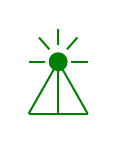
\begin{tikzpicture} [scale=0.75]
        \draw [line width=0.25mm, green!50!black] (2, -0.44) to (2.5,0.44);
        \draw [line width=0.25mm, green!50!black] (3, -0.44) to (2.5,0.44);
        \draw [line width=0.25mm, green!50!black] (2, -0.44) to (3,-0.44);
        \draw [line width=0.25mm, green!50!black] (2.5, -0.44) to (2.5,0.44);
        \draw [fill=green!50!black, green!50!black] (2.5,0.44) circle(1.5mm);

        \draw [line width=0.25mm, green!50!black] (2.5, 0.725) to (2.5,1.0);
        \draw [line width=0.25mm, green!50!black] (2.65, 0.65) to (2.825,0.85);
        \draw [line width=0.25mm, green!50!black] (2.725, 0.44) to (3,0.44);
        \draw [line width=0.25mm, green!50!black] (2.35, 0.65) to (2.175,0.85);
        \draw [line width=0.25mm, green!50!black] (2.275, 0.44) to (2,0.44);

        \end{tikzpicture}
    };
    %()
    \draw[fill=green!50!black, green!50!black] (-0.25,-2.15) circle (0.025);
    \draw[fill=green!50!black, green!50!black] (0,-2.15) circle (0.025);
    \draw[fill=green!50!black, green!50!black] (0.25,-2.15) circle (0.025);
    %
    \node (dataRadio2) [right=of dataRadio1] %, xshift=-1.5mm
    {
        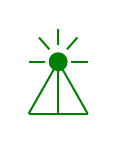
\begin{tikzpicture} [scale=0.75]
        \draw [line width=0.25mm, green!50!black] (2, -0.44) to (2.5,0.44);
        \draw [line width=0.25mm, green!50!black] (3, -0.44) to (2.5,0.44);
        \draw [line width=0.25mm, green!50!black] (2, -0.44) to (3,-0.44);
        \draw [line width=0.25mm, green!50!black] (2.5, -0.44) to (2.5,0.44);
        \draw [fill=green!50!black, green!50!black] (2.5,0.44) circle(1.5mm);

        \draw [line width=0.25mm, green!50!black] (2.5, 0.725) to (2.5,1.0);
        \draw [line width=0.25mm, green!50!black] (2.65, 0.65) to (2.825,0.85);
        \draw [line width=0.25mm, green!50!black] (2.725, 0.44) to (3,0.44);
        \draw [line width=0.25mm, green!50!black] (2.35, 0.65) to (2.175,0.85);
        \draw [line width=0.25mm, green!50!black] (2.275, 0.44) to (2,0.44);

        \end{tikzpicture}
    };%fill=green!50!black,
    \draw[line width=0.25mm, green!25!black] (0.25,-1) circle (3);
\end{tikzpicture}
};
    \draw (1.5, 4) node {\begin{tikzpicture}[scale=0.375, transform shape]
    \node (controlRadio)
    {
        \begin{tikzpicture} [scale=1.0]
        \draw [fill=blue!25!white, blue!75!black] (2.3, -0.44) -- (2.5,0.44) -- (2.7, -0.44);
        \draw [fill=blue!25!white, blue!75!black] (2.5,0.44) circle(1.5mm);

        \draw [line width=0.25mm, blue!25!white] (2.5, 0.725) to (2.5,1.0);
        \draw [line width=0.25mm, blue!25!white] (2.65, 0.65) to (2.825,0.85);
        \draw [line width=0.25mm, blue!25!white] (2.725, 0.44) to (3,0.44);
        \draw [line width=0.25mm, blue!25!white] (2.35, 0.65) to (2.175,0.85);
        \draw [line width=0.25mm, blue!25!white] (2.275, 0.44) to (2,0.44);

        \end{tikzpicture}
    };
    \node (dataRadio1) [below=of controlRadio, xshift=-1.0cm, yshift=0.5cm] %, xshift=-1.5mm
    {
        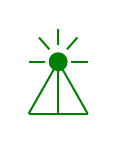
\begin{tikzpicture} [scale=0.75]
        \draw [line width=0.25mm, green!50!black] (2, -0.44) to (2.5,0.44);
        \draw [line width=0.25mm, green!50!black] (3, -0.44) to (2.5,0.44);
        \draw [line width=0.25mm, green!50!black] (2, -0.44) to (3,-0.44);
        \draw [line width=0.25mm, green!50!black] (2.5, -0.44) to (2.5,0.44);
        \draw [fill=green!50!black, green!50!black] (2.5,0.44) circle(1.5mm);

        \draw [line width=0.25mm, green!50!black] (2.5, 0.725) to (2.5,1.0);
        \draw [line width=0.25mm, green!50!black] (2.65, 0.65) to (2.825,0.85);
        \draw [line width=0.25mm, green!50!black] (2.725, 0.44) to (3,0.44);
        \draw [line width=0.25mm, green!50!black] (2.35, 0.65) to (2.175,0.85);
        \draw [line width=0.25mm, green!50!black] (2.275, 0.44) to (2,0.44);

        \end{tikzpicture}
    };
    %()
    \draw[fill=green!50!black, green!50!black] (-0.25,-2.15) circle (0.025);
    \draw[fill=green!50!black, green!50!black] (0,-2.15) circle (0.025);
    \draw[fill=green!50!black, green!50!black] (0.25,-2.15) circle (0.025);
    %
    \node (dataRadio2) [right=of dataRadio1] %, xshift=-1.5mm
    {
        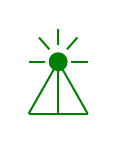
\begin{tikzpicture} [scale=0.75]
        \draw [line width=0.25mm, green!50!black] (2, -0.44) to (2.5,0.44);
        \draw [line width=0.25mm, green!50!black] (3, -0.44) to (2.5,0.44);
        \draw [line width=0.25mm, green!50!black] (2, -0.44) to (3,-0.44);
        \draw [line width=0.25mm, green!50!black] (2.5, -0.44) to (2.5,0.44);
        \draw [fill=green!50!black, green!50!black] (2.5,0.44) circle(1.5mm);

        \draw [line width=0.25mm, green!50!black] (2.5, 0.725) to (2.5,1.0);
        \draw [line width=0.25mm, green!50!black] (2.65, 0.65) to (2.825,0.85);
        \draw [line width=0.25mm, green!50!black] (2.725, 0.44) to (3,0.44);
        \draw [line width=0.25mm, green!50!black] (2.35, 0.65) to (2.175,0.85);
        \draw [line width=0.25mm, green!50!black] (2.275, 0.44) to (2,0.44);

        \end{tikzpicture}
    };%fill=green!50!black,
    \draw[line width=0.25mm, green!25!black] (0.25,-1) circle (3);
\end{tikzpicture}
};
    \draw (2.5, 1) node {\begin{tikzpicture}[scale=0.375, transform shape]
    \node (controlRadio)
    {
        \begin{tikzpicture} [scale=1.0]
        \draw [fill=blue!25!white, blue!75!black] (2.3, -0.44) -- (2.5,0.44) -- (2.7, -0.44);
        \draw [fill=blue!25!white, blue!75!black] (2.5,0.44) circle(1.5mm);

        \draw [line width=0.25mm, blue!25!white] (2.5, 0.725) to (2.5,1.0);
        \draw [line width=0.25mm, blue!25!white] (2.65, 0.65) to (2.825,0.85);
        \draw [line width=0.25mm, blue!25!white] (2.725, 0.44) to (3,0.44);
        \draw [line width=0.25mm, blue!25!white] (2.35, 0.65) to (2.175,0.85);
        \draw [line width=0.25mm, blue!25!white] (2.275, 0.44) to (2,0.44);

        \end{tikzpicture}
    };
    \node (dataRadio1) [below=of controlRadio, xshift=-1.0cm, yshift=0.5cm] %, xshift=-1.5mm
    {
        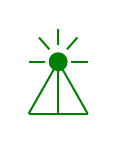
\begin{tikzpicture} [scale=0.75]
        \draw [line width=0.25mm, green!50!black] (2, -0.44) to (2.5,0.44);
        \draw [line width=0.25mm, green!50!black] (3, -0.44) to (2.5,0.44);
        \draw [line width=0.25mm, green!50!black] (2, -0.44) to (3,-0.44);
        \draw [line width=0.25mm, green!50!black] (2.5, -0.44) to (2.5,0.44);
        \draw [fill=green!50!black, green!50!black] (2.5,0.44) circle(1.5mm);

        \draw [line width=0.25mm, green!50!black] (2.5, 0.725) to (2.5,1.0);
        \draw [line width=0.25mm, green!50!black] (2.65, 0.65) to (2.825,0.85);
        \draw [line width=0.25mm, green!50!black] (2.725, 0.44) to (3,0.44);
        \draw [line width=0.25mm, green!50!black] (2.35, 0.65) to (2.175,0.85);
        \draw [line width=0.25mm, green!50!black] (2.275, 0.44) to (2,0.44);

        \end{tikzpicture}
    };
    %()
    \draw[fill=green!50!black, green!50!black] (-0.25,-2.15) circle (0.025);
    \draw[fill=green!50!black, green!50!black] (0,-2.15) circle (0.025);
    \draw[fill=green!50!black, green!50!black] (0.25,-2.15) circle (0.025);
    %
    \node (dataRadio2) [right=of dataRadio1] %, xshift=-1.5mm
    {
        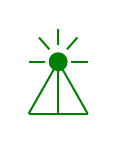
\begin{tikzpicture} [scale=0.75]
        \draw [line width=0.25mm, green!50!black] (2, -0.44) to (2.5,0.44);
        \draw [line width=0.25mm, green!50!black] (3, -0.44) to (2.5,0.44);
        \draw [line width=0.25mm, green!50!black] (2, -0.44) to (3,-0.44);
        \draw [line width=0.25mm, green!50!black] (2.5, -0.44) to (2.5,0.44);
        \draw [fill=green!50!black, green!50!black] (2.5,0.44) circle(1.5mm);

        \draw [line width=0.25mm, green!50!black] (2.5, 0.725) to (2.5,1.0);
        \draw [line width=0.25mm, green!50!black] (2.65, 0.65) to (2.825,0.85);
        \draw [line width=0.25mm, green!50!black] (2.725, 0.44) to (3,0.44);
        \draw [line width=0.25mm, green!50!black] (2.35, 0.65) to (2.175,0.85);
        \draw [line width=0.25mm, green!50!black] (2.275, 0.44) to (2,0.44);

        \end{tikzpicture}
    };%fill=green!50!black,
    \draw[line width=0.25mm, green!25!black] (0.25,-1) circle (3);
\end{tikzpicture}
};
    \draw (7.5, 1) node {\begin{tikzpicture}[scale=0.375, transform shape]
    \node (controlRadio)
    {
        \begin{tikzpicture} [scale=1.0]
        \draw [fill=blue!25!white, blue!75!black] (2.3, -0.44) -- (2.5,0.44) -- (2.7, -0.44);
        \draw [fill=blue!25!white, blue!75!black] (2.5,0.44) circle(1.5mm);

        \draw [line width=0.25mm, blue!25!white] (2.5, 0.725) to (2.5,1.0);
        \draw [line width=0.25mm, blue!25!white] (2.65, 0.65) to (2.825,0.85);
        \draw [line width=0.25mm, blue!25!white] (2.725, 0.44) to (3,0.44);
        \draw [line width=0.25mm, blue!25!white] (2.35, 0.65) to (2.175,0.85);
        \draw [line width=0.25mm, blue!25!white] (2.275, 0.44) to (2,0.44);

        \end{tikzpicture}
    };
    \node (dataRadio1) [below=of controlRadio, xshift=-1.0cm, yshift=0.5cm] %, xshift=-1.5mm
    {
        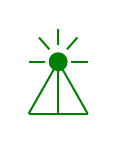
\begin{tikzpicture} [scale=0.75]
        \draw [line width=0.25mm, green!50!black] (2, -0.44) to (2.5,0.44);
        \draw [line width=0.25mm, green!50!black] (3, -0.44) to (2.5,0.44);
        \draw [line width=0.25mm, green!50!black] (2, -0.44) to (3,-0.44);
        \draw [line width=0.25mm, green!50!black] (2.5, -0.44) to (2.5,0.44);
        \draw [fill=green!50!black, green!50!black] (2.5,0.44) circle(1.5mm);

        \draw [line width=0.25mm, green!50!black] (2.5, 0.725) to (2.5,1.0);
        \draw [line width=0.25mm, green!50!black] (2.65, 0.65) to (2.825,0.85);
        \draw [line width=0.25mm, green!50!black] (2.725, 0.44) to (3,0.44);
        \draw [line width=0.25mm, green!50!black] (2.35, 0.65) to (2.175,0.85);
        \draw [line width=0.25mm, green!50!black] (2.275, 0.44) to (2,0.44);

        \end{tikzpicture}
    };
    %()
    \draw[fill=green!50!black, green!50!black] (-0.25,-2.15) circle (0.025);
    \draw[fill=green!50!black, green!50!black] (0,-2.15) circle (0.025);
    \draw[fill=green!50!black, green!50!black] (0.25,-2.15) circle (0.025);
    %
    \node (dataRadio2) [right=of dataRadio1] %, xshift=-1.5mm
    {
        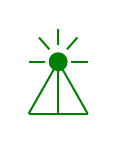
\begin{tikzpicture} [scale=0.75]
        \draw [line width=0.25mm, green!50!black] (2, -0.44) to (2.5,0.44);
        \draw [line width=0.25mm, green!50!black] (3, -0.44) to (2.5,0.44);
        \draw [line width=0.25mm, green!50!black] (2, -0.44) to (3,-0.44);
        \draw [line width=0.25mm, green!50!black] (2.5, -0.44) to (2.5,0.44);
        \draw [fill=green!50!black, green!50!black] (2.5,0.44) circle(1.5mm);

        \draw [line width=0.25mm, green!50!black] (2.5, 0.725) to (2.5,1.0);
        \draw [line width=0.25mm, green!50!black] (2.65, 0.65) to (2.825,0.85);
        \draw [line width=0.25mm, green!50!black] (2.725, 0.44) to (3,0.44);
        \draw [line width=0.25mm, green!50!black] (2.35, 0.65) to (2.175,0.85);
        \draw [line width=0.25mm, green!50!black] (2.275, 0.44) to (2,0.44);

        \end{tikzpicture}
    };%fill=green!50!black,
    \draw[line width=0.25mm, green!25!black] (0.25,-1) circle (3);
\end{tikzpicture}
};
    \draw (8.5, 4) node {\begin{tikzpicture}[scale=0.375, transform shape]
    \node (controlRadio)
    {
        \begin{tikzpicture} [scale=1.0]
        \draw [fill=blue!25!white, blue!75!black] (2.3, -0.44) -- (2.5,0.44) -- (2.7, -0.44);
        \draw [fill=blue!25!white, blue!75!black] (2.5,0.44) circle(1.5mm);

        \draw [line width=0.25mm, blue!25!white] (2.5, 0.725) to (2.5,1.0);
        \draw [line width=0.25mm, blue!25!white] (2.65, 0.65) to (2.825,0.85);
        \draw [line width=0.25mm, blue!25!white] (2.725, 0.44) to (3,0.44);
        \draw [line width=0.25mm, blue!25!white] (2.35, 0.65) to (2.175,0.85);
        \draw [line width=0.25mm, blue!25!white] (2.275, 0.44) to (2,0.44);

        \end{tikzpicture}
    };
    \node (dataRadio1) [below=of controlRadio, xshift=-1.0cm, yshift=0.5cm] %, xshift=-1.5mm
    {
        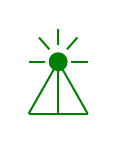
\begin{tikzpicture} [scale=0.75]
        \draw [line width=0.25mm, green!50!black] (2, -0.44) to (2.5,0.44);
        \draw [line width=0.25mm, green!50!black] (3, -0.44) to (2.5,0.44);
        \draw [line width=0.25mm, green!50!black] (2, -0.44) to (3,-0.44);
        \draw [line width=0.25mm, green!50!black] (2.5, -0.44) to (2.5,0.44);
        \draw [fill=green!50!black, green!50!black] (2.5,0.44) circle(1.5mm);

        \draw [line width=0.25mm, green!50!black] (2.5, 0.725) to (2.5,1.0);
        \draw [line width=0.25mm, green!50!black] (2.65, 0.65) to (2.825,0.85);
        \draw [line width=0.25mm, green!50!black] (2.725, 0.44) to (3,0.44);
        \draw [line width=0.25mm, green!50!black] (2.35, 0.65) to (2.175,0.85);
        \draw [line width=0.25mm, green!50!black] (2.275, 0.44) to (2,0.44);

        \end{tikzpicture}
    };
    %()
    \draw[fill=green!50!black, green!50!black] (-0.25,-2.15) circle (0.025);
    \draw[fill=green!50!black, green!50!black] (0,-2.15) circle (0.025);
    \draw[fill=green!50!black, green!50!black] (0.25,-2.15) circle (0.025);
    %
    \node (dataRadio2) [right=of dataRadio1] %, xshift=-1.5mm
    {
        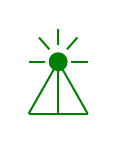
\begin{tikzpicture} [scale=0.75]
        \draw [line width=0.25mm, green!50!black] (2, -0.44) to (2.5,0.44);
        \draw [line width=0.25mm, green!50!black] (3, -0.44) to (2.5,0.44);
        \draw [line width=0.25mm, green!50!black] (2, -0.44) to (3,-0.44);
        \draw [line width=0.25mm, green!50!black] (2.5, -0.44) to (2.5,0.44);
        \draw [fill=green!50!black, green!50!black] (2.5,0.44) circle(1.5mm);

        \draw [line width=0.25mm, green!50!black] (2.5, 0.725) to (2.5,1.0);
        \draw [line width=0.25mm, green!50!black] (2.65, 0.65) to (2.825,0.85);
        \draw [line width=0.25mm, green!50!black] (2.725, 0.44) to (3,0.44);
        \draw [line width=0.25mm, green!50!black] (2.35, 0.65) to (2.175,0.85);
        \draw [line width=0.25mm, green!50!black] (2.275, 0.44) to (2,0.44);

        \end{tikzpicture}
    };%fill=green!50!black,
    \draw[line width=0.25mm, green!25!black] (0.25,-1) circle (3);
\end{tikzpicture}
};
    
    \draw (5, 4.9) node {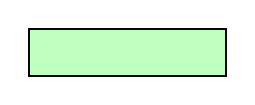
\begin{tikzpicture}[scale=1.0, transform shape]
    \tikzstyle{every node} = [draw, shape = rectangle, node distance=0mm, minimum width=4mm, minimum height=6mm, fill=green!25!white]
    \node[draw=black, thick, minimum width=25mm] (channel1) {};
\end{tikzpicture}
};
    \draw (5, 4.2) node {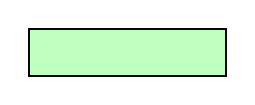
\begin{tikzpicture}[scale=1.0, transform shape]
    \tikzstyle{every node} = [draw, shape = rectangle, node distance=0mm, minimum width=4mm, minimum height=6mm, fill=green!25!white]
    \node[draw=black, thick, minimum width=25mm] (channel1) {};
\end{tikzpicture}
};
    \draw (5, 3.5) node {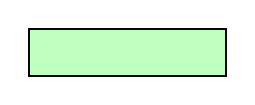
\begin{tikzpicture}[scale=1.0, transform shape]
    \tikzstyle{every node} = [draw, shape = rectangle, node distance=0mm, minimum width=4mm, minimum height=6mm, fill=green!25!white]
    \node[draw=black, thick, minimum width=25mm] (channel1) {};
\end{tikzpicture}
};
    \draw (5, 2.8) node {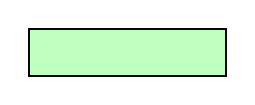
\begin{tikzpicture}[scale=1.0, transform shape]
    \tikzstyle{every node} = [draw, shape = rectangle, node distance=0mm, minimum width=4mm, minimum height=6mm, fill=green!25!white]
    \node[draw=black, thick, minimum width=25mm] (channel1) {};
\end{tikzpicture}
};%[label=below:{\tiny \(n\) spectrum channels}]
    \draw (5, 1.25) node {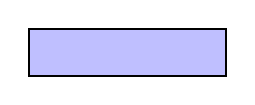
\begin{tikzpicture}[scale=1.0, transform shape]
    \tikzstyle{every node} = [draw, shape = rectangle, node distance=0mm, minimum width=4mm, minimum height=6mm, fill=blue!25!white]
    \node[draw=black, thick, minimum width=25mm] (channel1) {};
\end{tikzpicture}
};%[label=below:{\tiny dedicated control channel}]
\end{tikzpicture}
};
\end{tikzpicture}
\caption{System model of a CMRN}
\label{fig:systemmodel}
\end{center}
\vspace{-0.5cm}
\end{figure}

Under the presented system model, our research question is how to efficiently use the available multiple data transmission radios to get enhanced total network throughput while limiting end-to-end delay. As there is no central authority in the considered system model, solution of the problem must be distributed. Besides, the decision making must also be online as the primary and secondary users' behavior can dynamically vary and thus can not be predicted beforehand. Considering these aspects, we propose a new solution in the next section.

\section{Feedback-based Multi-radio Exploitation Approach}
\label{sec:feedback}

Our proposed approach consists of mainly two different types of feedbacks. Firstly, we measure packet transmission ratio for each radio to evaluate radio performance. Secondly, we calculate channel utilization ratio for each channel to assess corresponding channel condition.

\subsection{Overview of The Proposed Approach}

We present a brief overview of our proposed feedback-based approach in Fig.~\ref{fig:overview}. As SUs are equipped with multiple radios, a single radio is first selected to send an Data Link layer packet. The radio selection process as described in Section~\ref{subsec:radioSelect} is based on packet transmission ratio. The selected radio then senses the PU activity on its current channel. If the current channel is idle, it transmits the packet following an standard CSMA-CA protocol. However, if the current channel is busy, then the radio selects another channel and starts switching to that channel. The channel selection process is based on channel utilization ratio and is described in Section~\ref{subsec:channelSelect}.

\begin{figure}[!htb]
\begin{center}
%\resizebox{0.625\textwidth}{!}{
\begin{center}
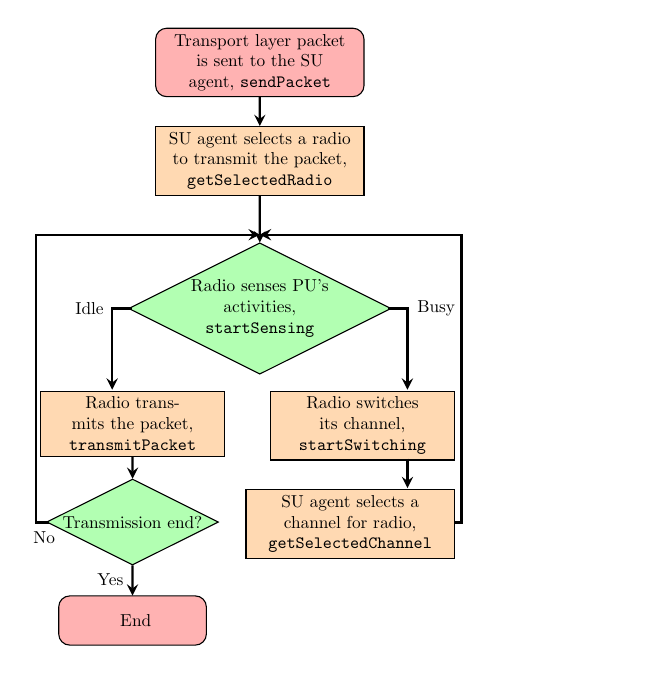
\begin{tikzpicture}[node distance=2cm, scale=0.625, transform shape]
\tikzset{every node/.style={text width=4cm}}
\tikzstyle{startstop} = [rectangle, rounded corners, minimum width=3cm, minimum height=1cm,text centered, draw=black, fill=red!30]
\tikzstyle{io} = [trapezium, trapezium left angle=70, trapezium right angle=110, minimum width=3cm, minimum height=1cm, text centered, draw=black, fill=blue!30]
\tikzstyle{process} = [rectangle, minimum width=3cm, minimum height=1cm, text centered, draw=black, fill=orange!30]
\tikzstyle{decision} = [diamond, minimum width=1cm,  text badly centered, inner sep=0pt, draw=black, fill=green!30]
\tikzstyle{arrow} = [thick,->,>=stealth]
\node (sendPacket) [startstop] {Transport layer packet is sent to the SU agent, \texttt{sendPacket}};
\node (getSelectedRadio) [process, below of=sendPacket] {SU agent selects a radio to transmit the packet, \texttt{getSelectedRadio}};
\node (startSensing) [decision, text width=3cm, aspect=2, below of=getSelectedRadio, yshift=-1cm] {Radio senses PU's activities, \texttt{startSensing}};
\node (startSwitching) [process, text width=3.5cm, below right =1cm and -0.625 cm of startSensing, xshift=-0.5cm] {Radio switches its channel, \texttt{startSwitching}};
%right of=startSensing, yshift=-3cm
\node (getSelectedChannel) [process, below of=startSwitching, xshift=-0.25cm] {SU agent selects a channel for radio, \texttt{getSelectedChannel}};
\node (transmitPacket) [process, text width=3.5cm, below left =1cm and -0.625 cm of startSensing] {Radio transmits the packet, \texttt{transmitPacket}};
\node (endTransmit) [decision, text width=3cm, aspect=2, below of=transmitPacket] {Transmission end?};
\node (end) [startstop, text width=0.5cm, below of=endTransmit] {End};
\draw [arrow] (sendPacket) -- (getSelectedRadio);
\draw [arrow] (getSelectedRadio) -- (startSensing);
\draw [arrow] (transmitPacket) -- (endTransmit);
\draw [arrow] (endTransmit) -- (end);
\node at (-2.6, -9.65) {No};
\node at (-1.3, -10.5) {Yes};
\node at (-1.75, -5) {Idle};
\node at (5.2, -5) {Busy};
\draw [arrow] (-4.28,-9.35) -- (-4.55,-9.35) -- (-4.55, -3.5) -- (0, -3.5);
\draw [arrow] (-2.6,-5) -- (-3,-5) -- (-3,-6.65);
\draw [arrow] (2.6,-5) -- (3,-5) -- (3,-6.65);
\draw [arrow] (3,-8.05) --  (3,-8.65);
\draw [arrow] (3.95,-9.35) -- (4.1,-9.35) -- (4.1, -3.5) -- (0, -3.5);
\end{tikzpicture}
\end{center}
%}
\caption{High-level overview of the proposed approach}
\label{fig:overview}
\end{center}
\vspace{-1cm}
\end{figure}

\iffalse
\begin{figure}[!htb]
\begin{center}
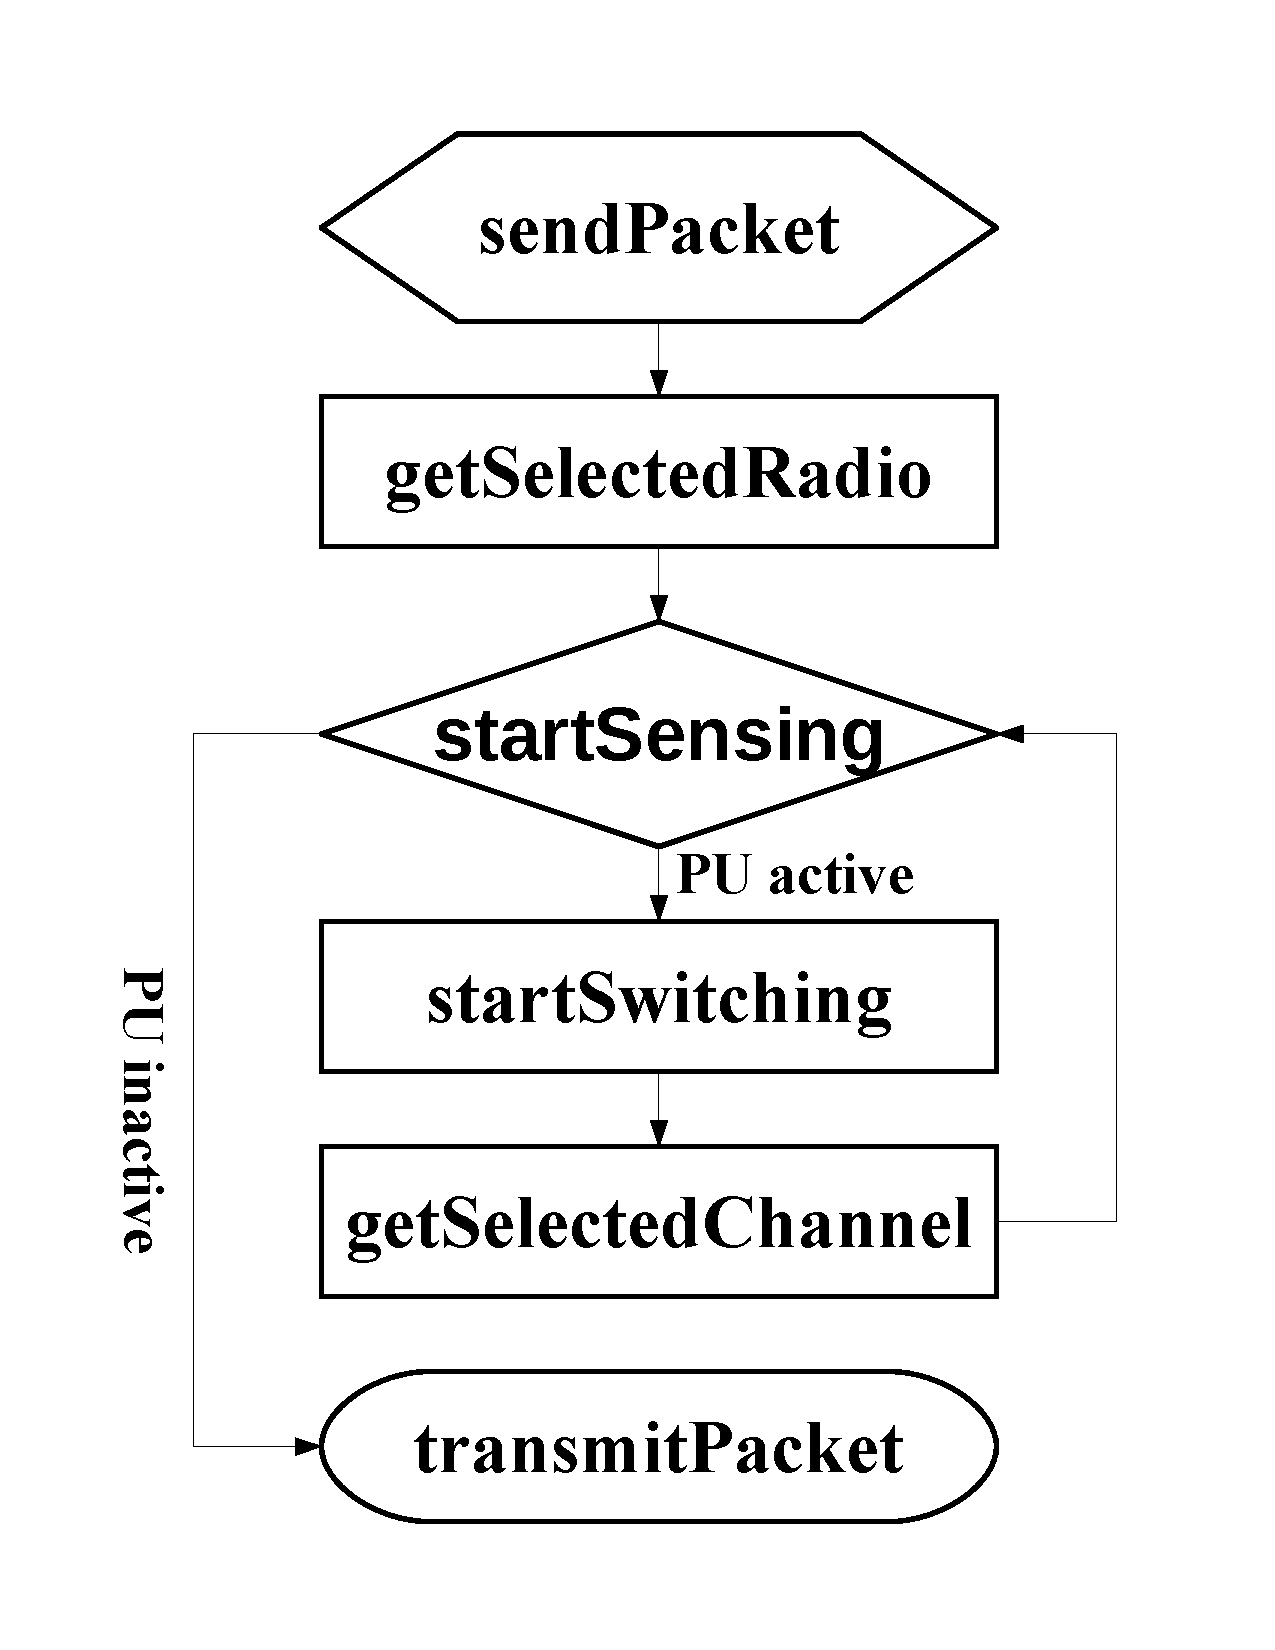
\includegraphics[scale=0.25]{flowchart}
\caption{High-level overview of the proposed mechanism}
\label{fig:overview}
\end{center}
\end{figure}
\fi

\subsection{Radio Selection Based on Packet Transmission Ratio}
\label{subsec:radioSelect}

When SUs are equipped with multiple data transmission radios, the first issue comes into play is to select the radio for transmitting data packets. For this selection, our proposed approach maintains two counters for each radio namely \texttt{pktQueued} denoting the number of packets queued for the radio and \texttt{pktSent} denoting the number of packets already transmitted by the radio. Whenever the Transport layer of an SU sends a packet for transmission to the lower layers, the secondary user agent calculates the ratio between \texttt{pktSent} and \texttt{pktQueued} for each radio. We define the ratio as Packet Transmission Ratio, \texttt{sentQueuedRatio}. Subsequently, we normalize values of the ratio to rank the radios in a uniform manner. A larger value of such packet transmission ratio implies that the corresponding radio has been successful to transmit more packets than others. Using these packet transmission ratios as the weights, our proposed approach conducts a weighted lottery to select radios for transmission of packets.

At the beginning of the packet transmission process, an SU's radio senses its current channel. If the cognitive radio finds that the current channel is busy, then the radio starts a channel switching process. At the beginning of the channel switching process, the SU agent lists all the channels currently not used by any radio of the corresponding SU. If no such channel can be found, the radio is reported as Off and the queued packets are discarded as dropped. Otherwise, a channel is selected from the list of available channels, \texttt{availableChannels} based on current channel utilization ratio. We present the selection process along with the definition of the channel utilization ratio next.

\subsection{Channel Selection Based on Channel Utilization Ratio}
\label{subsec:channelSelect}

In our proposed approach, each SU maintains a list of currently used channels, \texttt{currentChannels} and currently available channels, \texttt{availableChannels}. These lists denote the current channel occupancy of the SU's radios and the channels currently not used by any radio correspondingly. Using these channel lists, multiple radios within an SU co-ordinate to avoid intra-user radio collision. Each SU keeps two counters for each channel. First, \texttt{pktTransmitted} counts the number of packets transmitted in the channel by the corresponding SU radios. Besides, \texttt{pktReceived} counts the number of packets successfully received by the corresponding receiver. The counter, \texttt{pktReceived} is incremented after reception of each acknowledgment packet. When a switching radio requires selecting a channel among \texttt{availableChannels}, the SU agent calculates the ratio between \texttt{pktReceived} and \texttt{pktTransmitted} for each channel on the list, \texttt{availableChannels}. We define the ratio as Channel Utilization Ratio, \texttt{RxTxRatio}. We normalize this ratio to rank the channels in a uniform manner. Using these channel utilization ratios as the weights, the SU agent conducts a weighted lottery to select the channel to switch over.

The last two important aspects of our feedback-based multi-radio exploitation approach are the reactivation of Off radios and probabilistic channel switching. Radios marked Off at the beginning of a channel switching process, are reactivated probabilistically by the radio selection process. While calculating packet transmission ratio from \texttt{pktSent} and \texttt{pktQueued}, in the case of Off radios, the ratio is multiplied by \texttt{wakeUpProbability} to make it less likely to be selected as the next radio for sending a packet. Though, if selected, the Off radio is reported as On and it starts its cognitive cycle through the channel sensing process. The probabilistic channel switching implies that radios do not always switch after finding their current channel busy. The channel switching process occurs at a probability of \texttt{switchingProbability}.

{
\begin{algorithm}
\scriptsize
\caption{$\mathit{sendPacket}$: SU agent sending a packet, $p$}
\label{alg:sendPacket}
\begin{algorithmic}[1]
\Function{$\mathit{sendPacket}$}{}
\State $\mathit{radioIndex}\gets \mathit{getSelectedRadio}()$
\State $pktQueued[radioIndex]\gets $\Statex$ 1+\mathit{pktQueued}[\mathit{radioIndex}]$
\State $\mathit{radioStatus}[\mathit{radioIndex}]\gets \mathit{On}$
\State $\mathit{startSensing}(\mathit{radioIndex})$
\EndFunction
\end{algorithmic}
\end{algorithm}
\vspace{-0.6cm}
\begin{algorithm}
\scriptsize
\caption{$\mathit{startSensing}$: SU's radio sensing its channel}
\label{alg:startSensing}
\begin{algorithmic}[1]
\Function{$\mathit{startSensing}$}{$\mathit{radioIndex}$}
\If{$\mathit{currentChannel}[\mathit{radioIndex}]$ is $\mathit{Busy}$}
\State $\mathit{startSwitching}(\mathit{radioIndex})$
\Else
\State $\mathit{transmitPacket}(\mathit{radioIndex})$
\EndIf
\EndFunction
\end{algorithmic}
\end{algorithm}
\vspace{-0.6cm}
\begin{algorithm}
\scriptsize
\caption{$\mathit{startSwitching}$: SU's radio changing its channel}\label{alg:startSwitching}
\begin{algorithmic}[1]
\Function{$\mathit{startSwitching}$}{$\mathit{radioIndex}$}
\State Stop the switching process and \textbf{return} with the probability $(1-\mathit{switchingProbability})$
\State $\mathit{availableChannels} \gets $ all the channels currently not used by any radio of the SU
\If{$\mathit{availableChannels}=\varnothing$}
\State $\mathit{radioStatus}[\mathit{radioIndex}]\gets \mathit{Off}$
\State $\mathit{dropPacket}()$
\Else
\State $\mathit{channelIndex}\gets$\Statex$ \mathit{getSelectedChannel}(\mathit{availableChannels})$
\State $\mathit{currentChannel}[\mathit{radioIndex}] \gets \mathit{channelIndex}$
\State $\mathit{channels}[\mathit{channelIndex}] \gets \mathit{Used}$
\State $\mathit{startSensing}(\mathit{radioIndex})$
\EndIf
\EndFunction
\end{algorithmic}
\end{algorithm}
\vspace{-0.5cm}
\begin{algorithm}
\scriptsize
\caption{$\mathit{transmitPacket}$: SU's radio transmitting a packet, $p$}
\label{alg:transmitPacket}
\begin{algorithmic}[1]
\Function{$\mathit{transmitPacket}$}{$\mathit{radioIndex}$}
\State $\mathit{pktSent}[\mathit{radioIndex}]\gets \mathit{pktSent}[\mathit{radioIndex}]+1$
\State $\mathit{pktTransmitted}[\mathit{currentChannel}[\mathit{radioIndex}]]\gets$\par\hskip\algorithmicindent$\mathit{pktTransmitted}[\mathit{currentChannel}[\mathit{radioIndex}]]$\par\hskip\algorithmicindent$+1$
\State encapsulate $\mathit{radioIndex}$ within the packet, $p$ and transmit it following CSMA-CA
\EndFunction
\end{algorithmic}
\end{algorithm}
\vspace{-0.25cm}
\begin{algorithm}
\scriptsize
\caption{$\mathit{receiveAckPacket}$: SU's radio receiving an Ack packet, $p$}
\label{alg:receivePacket}
\begin{algorithmic}[1]
\Function{$\mathit{receivePacket}$}{$p$}
\State $\mathit{radioIndex} \gets $ the radio index extracted from the packet
\If{$\mathit{radioIndex}=$ current radio's index}
\State $\mathit{pktReceivedRadio}[\mathit{radioIndex}]\gets$\Statex$ \mathit{pktReceivedRadio}[\mathit{radioIndex}]+1$
\State $\mathit{pktReceived}[\mathit{currentChannel}[\mathit{radioIndex}]]\gets$\Statex$ \mathit{pktReceived}[\mathit{currentChannel}[\mathit{radioIndex}]]+1$
\EndIf
\EndFunction
\end{algorithmic}
\end{algorithm}
\vspace{-0.25cm}
\begin{algorithm}
\scriptsize
\caption{$\mathit{getSelectedRadio}$: Selects an SU radio to send a packet}
\label{alg:getSelectedRadio}
\begin{algorithmic}[1]
\Function{$\mathit{getSelectedRadio}$}{}
%\State $\mathit{radios} \gets$ all the radios
\State $k \gets$ the number of radios
\State $\mathit{sentQueuedRatio} [0\ldots k] \gets $a new array of floating point values
\State $\mathit{total} \gets 0.0$
\For{$r=1$ \textbf{to} $k$}
\State $\mathit{sentQueuedRatio}[r] \gets \dfrac{(1+\mathit{pktSent}[\mathit{r}])}{(1+\mathit{pktQueued}[\mathit{r}])}$
\If{$\mathit{radioStatus}[\mathit{r}]=\mathit{Off}$}
\State $\mathit{sentQueuedRatio}[r] \gets$\Statex[2]$ \mathit{sentQueuedRatio}[r] \times \mathit{wakeUpProbability}$
\EndIf
\State $\mathit{total} \gets \mathit{total} + \mathit{sentQueuedRatio}[r]$
\EndFor
\For{$r=1$ \textbf{to} $k$}
\State $\mathit{sentQueuedRatio}[r] \gets \dfrac{\mathit{sentQueuedRatio}[r]}{\mathit{total}}$
\EndFor
\State $\mathit{radioIndex} \gets$ winner of the weighted lottery among all the radios with weight, $\mathit{sentQueuedRatio}$
\State \textbf{return} $\mathit{radioIndex}$
\EndFunction
\end{algorithmic}
\end{algorithm}
\vspace{-0.25cm}
\begin{algorithm}
\scriptsize
\caption{$\mathit{getSelectedChannel}$: Selects a new channel to switch for an SU radio over the $\mathit{availableChannels}$}
\label{alg:getSelectedRadio}
\begin{algorithmic}[1]
\Function{$\mathit{getSelectedChannel}$}{$\mathit{availableChannels}$}
\State $k \gets$ the number of channels in $\mathit{availableChannels}$
\State $\mathit{RxTxRatio} [0\ldots k] \gets $ a new array of floating point values
\State $\mathit{total} \gets 0.0$
\For{$r=1$ \textbf{to} $k$}
\State $\mathit{RxTxRatio}[r] \gets \dfrac{(1+\mathit{pktReceived}[\mathit{r}])}{(1+\mathit{pktTransmitted}[\mathit{r}])}$
\State $\mathit{total} \gets \mathit{total} + \mathit{RxTxRatio}[r]$
\EndFor
\For{$r=1$ \textbf{to} $k$}
\State $\mathit{RxTxRatio}[r] \gets \dfrac{\mathit{RxTxRatio}[r]}{\mathit{total}}$
\EndFor
\State $\mathit{channelIndex} \gets$ winner of the weighted lottery among all the channels in $\mathit{availableChannels}$ with weight, $\mathit{RxTxRatio}$
\State \textbf{return} $\mathit{channelIndex}$
\EndFunction
\end{algorithmic}
\end{algorithm}
%\vspace{-0.1cm}
}

\subsection{Sequential Radio and Channel Selection}

An important characteristic of our proposed approach is the sequential radio and channel selection (as described in Figure~\ref{fig:blockDiagram}) instead of jointly optimized radio-channel selection. In our approach, when transport layer packets come in the data link layer, our SU agent enqueue them to one of the available radio's queue. Our packet transmission ratio based radio selection algorithm (Subsection~\ref{subsec:radioSelect}) determines that on which radio's queue each packet will be enqueued. During this time, the channel through which this packet will be transmitted is not decided. The channel selection decision is made later when the packet is dequeued from the radio's queue. At that time if the radio senses no primary user on the radio's currently assigned channel, the dequeued packet is transmitted using the currently assigned channel. Only if the radio's sensing results show that there is primary user activity of the current channel, the radio switches from the current channel, only then the channel selection algorithm is used to find the new channel.

\begin{figure}[!htbp]
    \begin{center}
        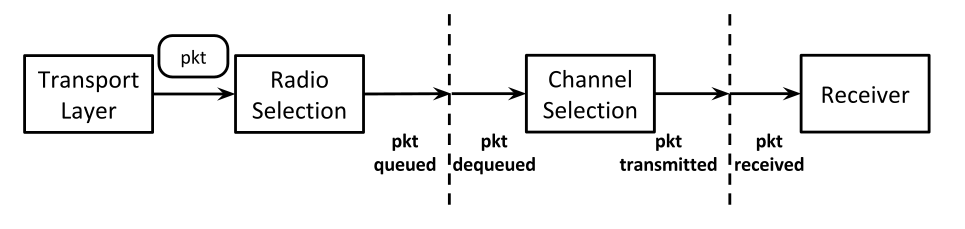
\includegraphics[width=0.5\textwidth]{blockDiagram.png}
        \caption{Operational pipeline of our proposed feedback-based multi-radio exploitation approach}
        \label{fig:blockDiagram}
    \end{center}
    \vspace{-1.0cm}
\end{figure}

The reason behind this sequential radio and channel selection is the dynamic nature of cognitive radio networks. When the packets are enqueued in the radio, neither the actual time when any of these packets will be transmitted nor the channels' state at that time can be accurately predicted. Therefore, any jointly optimized radio-channel selection could not consider the actual channel condition at the time of packet transmission. Keeping this issue in mind, our proposed approach employs sequential radio and channel selection process.

\subsection{Variants of Our Proposed Approach}

We create three variants of our proposed approach introducing radio and channel selection based on a random variable following a uniform distribution. While selecting the next radio for data packet transmission, we can randomly select any one of data radios ignoring the packet transmission ratios. Similarly, the next channel to switch can also be chosen randomly from the available channels irrespective of the channel utilization ratio. We define this random radio and channel selection policy as unweighted lottery. From this unweighted lottery, we devise three variants of our proposed approach as described in Table~\ref{tab:variantDefintion}. The approach of randomly selecting both the radio and the channel has not be listed as the variants of the proposed approach as that approach is quite similar to the approach proposed by Zhong et al.,~\cite{zhong2014capacity}.

\begin{table*}
\begin{center}
  \caption{Several variants of the proposed feedback-based approach}
  \label{tab:variantDefintion}
  \begin{tabular}{lll}
    \toprule
    Variant name & Radio selection policy & Channel selection policy\\
    \midrule
    Radio feedback & Weighted lottery based on radio transmission ratio & Unweighted lottery \\
    Channel feedback & Unweighted lottery  & Weighted lottery based on channel utilization ratio \\
    Radio channel feedback & Weighted lottery based on radio transmission ratio & Weighted lottery based on channel utilization ratio \\
    \bottomrule
  \end{tabular}
\end{center}
\vspace{-0.5cm}
\end{table*}



\section{Experimental Evaluation}
\label{sec:results}

Our proposed system requires wireless devices with multiple networking interface modules. Each of these modules must also have cognitive capability to ensure the basic requirements of our proposed architecture. The development of such devices involves a highly complex level of sophistication and fabrication. Such a development of cognitive radio networks in real setup is still under research. Therefore, we evaluate the performance of our proposed feedback-based multi-radio exploitation approach through extensive discrete-event simulation using ns-3.

We implement our proposed approach on top of the Cognitive radio extension for ns-3 namely CRE-NS3~\cite{al2014simulating}. We modify the cognitive module of CRE-NS3 to incorporate our feedback-based approach. The existing cognitive module of CRE-NS3 provides three interfaces for each device namely control interface, transmitter interface, and receiver interface. The transmitter and receiver interfaces of the module emulate a real cognitive transceivers. Therefore, we introduce the functionality of varying number of cognitive transceivers through varying the number of the transmitter and receiver interfaces.

Using the modified simulator, we implement our proposed approach and evaluate its performance on the basis of four performance metrics -- total network throughput, end-to-end delay, packet drop ratio, and application layer packet delivery ratio. Besides, we measure values of these metrics for two existing CMRN protocols and compared them against that obtained using several variants of our proposed approach. We briefly describe our simulation settings below before presenting the evaluation results.

\vspace{-0.4cm}
\subsection{Simulation Settings}
\vspace{-0.25cm}

We consider that arrival and departure of a PU follow a Poisson process~\cite{heo2008mathematical}. Accordingly, we consider an exponential distribution for both inter-arrival time and service time. Hence we adopt the mean time between two successive arrivals to be 5 seconds and the mean service time to be 2 seconds. Besides, we consider that each secondary user enables a constant bit rate application where the data transmission rate is varied from 1 Mbps to 32 Mbps. Here, each secondary user is equipped with a variable number of radios. Each of the radios consists of one transmitter interface and one receiver interface. The transmitter interface transmits data over any of the eleven orthogonal channels that conventionally operate with OFDM WiFi mode having 18Mbps data rate. For each transmitter interface or radio, we associate a drop-tail queue with a maximum capacity of 100 packets, each of 1KB in size. These interfaces have a transmission range of 130m and a sensing range of 250m. To ensure that the destination users are reachable from the source users, we place the destinations at an average distance of 80m from the sources. Maintaining such average distance, primary users and secondary users are placed randomly in an area of $500$m$\times 500$m. Here, we vary the number of secondary users from 12 to 40 with a granularity of 4. For each such settings, we perform 99 simulation iterations, each of 50 seconds, and then take average results of all the iterations. It is to be noted here that the maximum iteration count for obtaining 95\% confidence interval according to Monte Carlo Sampling~\cite{winston2000simulation} is found to be 61 in our experiment settings. 

We carefully set the tuning parameters of the proposed approach after numerous simulation trials. The channel switching probability of SU radios, \texttt{switchingProbability} was varied from 0.1 to 0.9 with a granularity of 0.05 and the reactivation probability of switched-off radios, \texttt{wakeUpProbability} was varied from 0.05 to 0.5 with a granularity of 0.05. Following these initial simulation results, we selected the value of these parameters that yielded best results in terms of throughput, delay, and packet drop ratio. The \texttt{switchingProbability} is set as 0.75 and the \texttt{wakeUpProbability} is set as 0.2. The channel sensing time for each of the cognitive radio is set as 0.01s while the channel switching time is set as 0.05s.

\vspace{-0.4cm}
\subsection{Simulation Results}
\vspace{-0.25cm}
\begin{figure*}[!htbp]
    \centering
    \begin{subfigure}[t]{0.45\textwidth}
        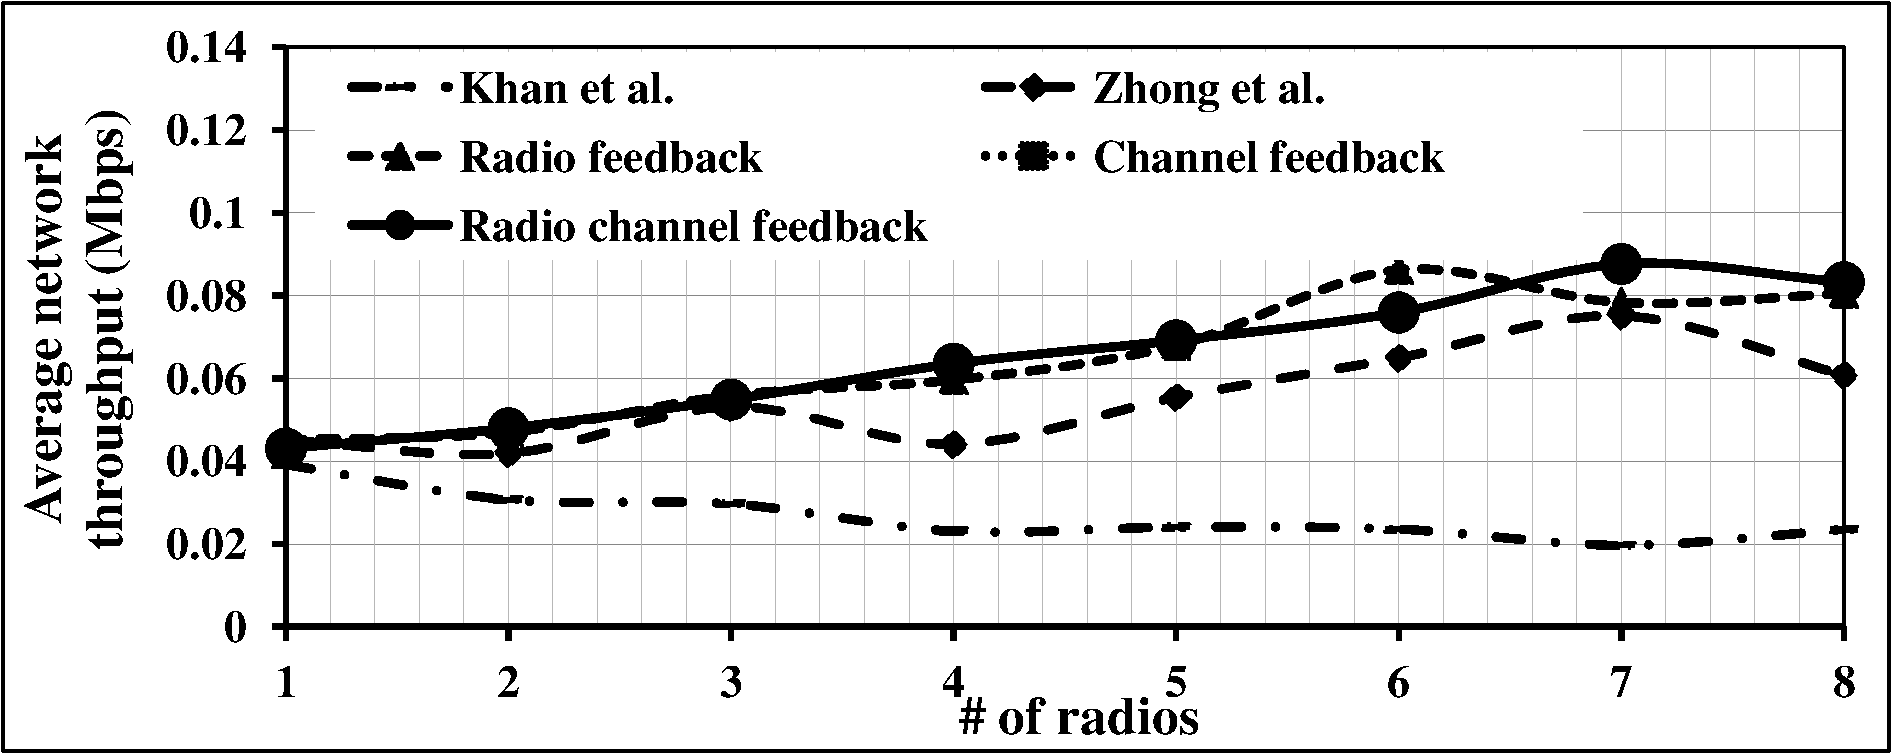
\includegraphics[width=\textwidth]{topology4/Throughput24d1}
        \caption{1Mbps application data rate}
        \label{fig:topology4T1}
    \end{subfigure}
    ~
    \begin{subfigure}[t]{0.45\textwidth}
        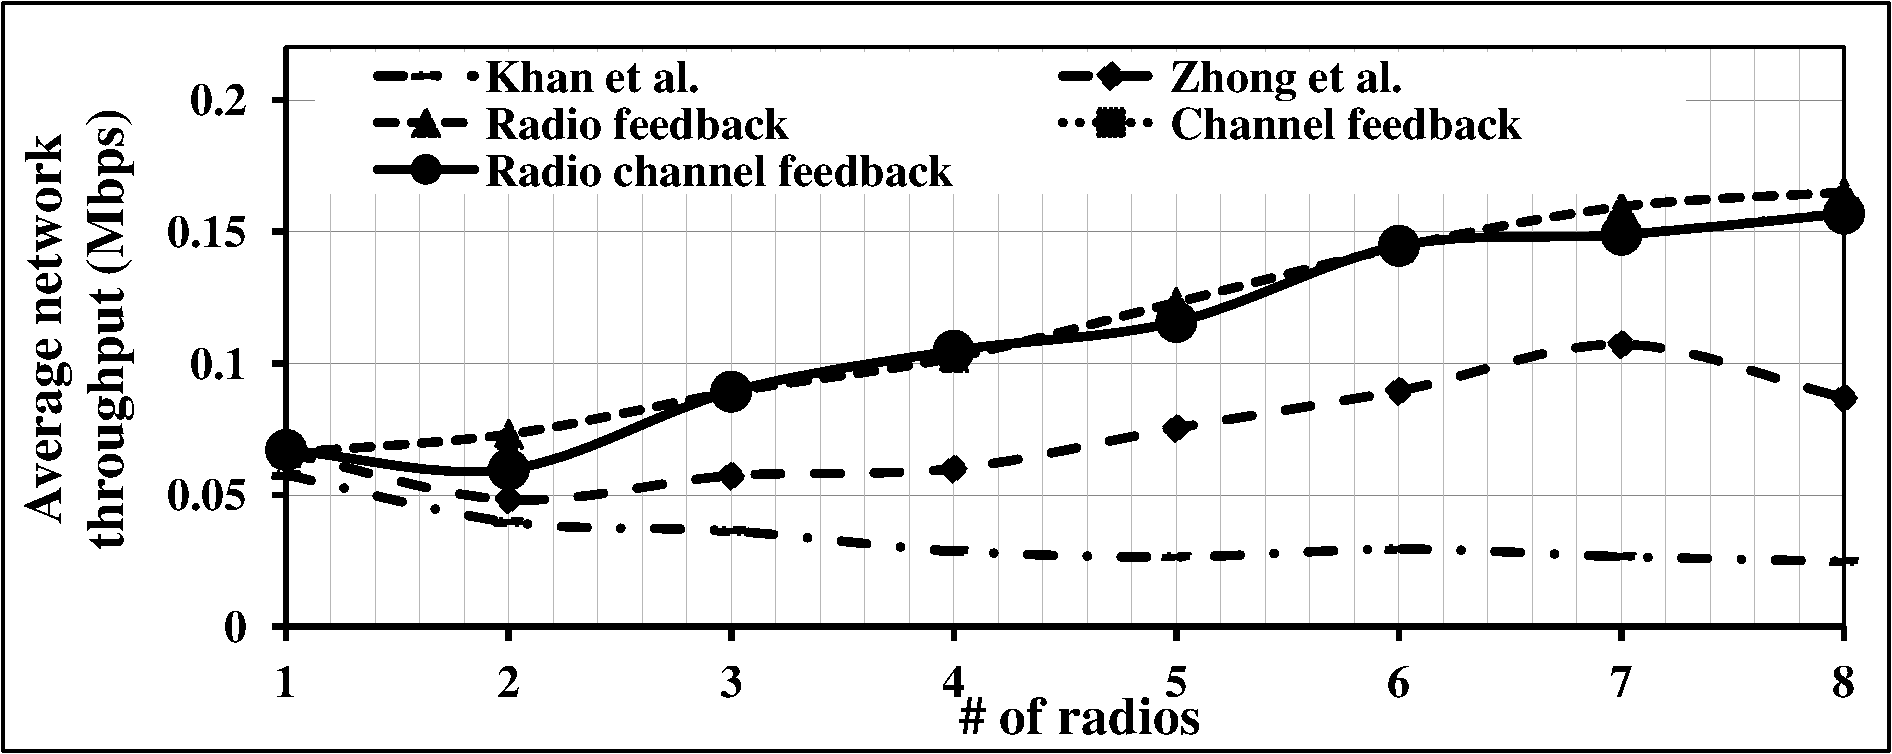
\includegraphics[width=\textwidth]{topology4/Throughput24d2}
        \caption{2Mbps application data rate}
        \label{fig:topology4T2}
    \end{subfigure}
    ~\\
    \begin{subfigure}[t]{0.45\textwidth}
        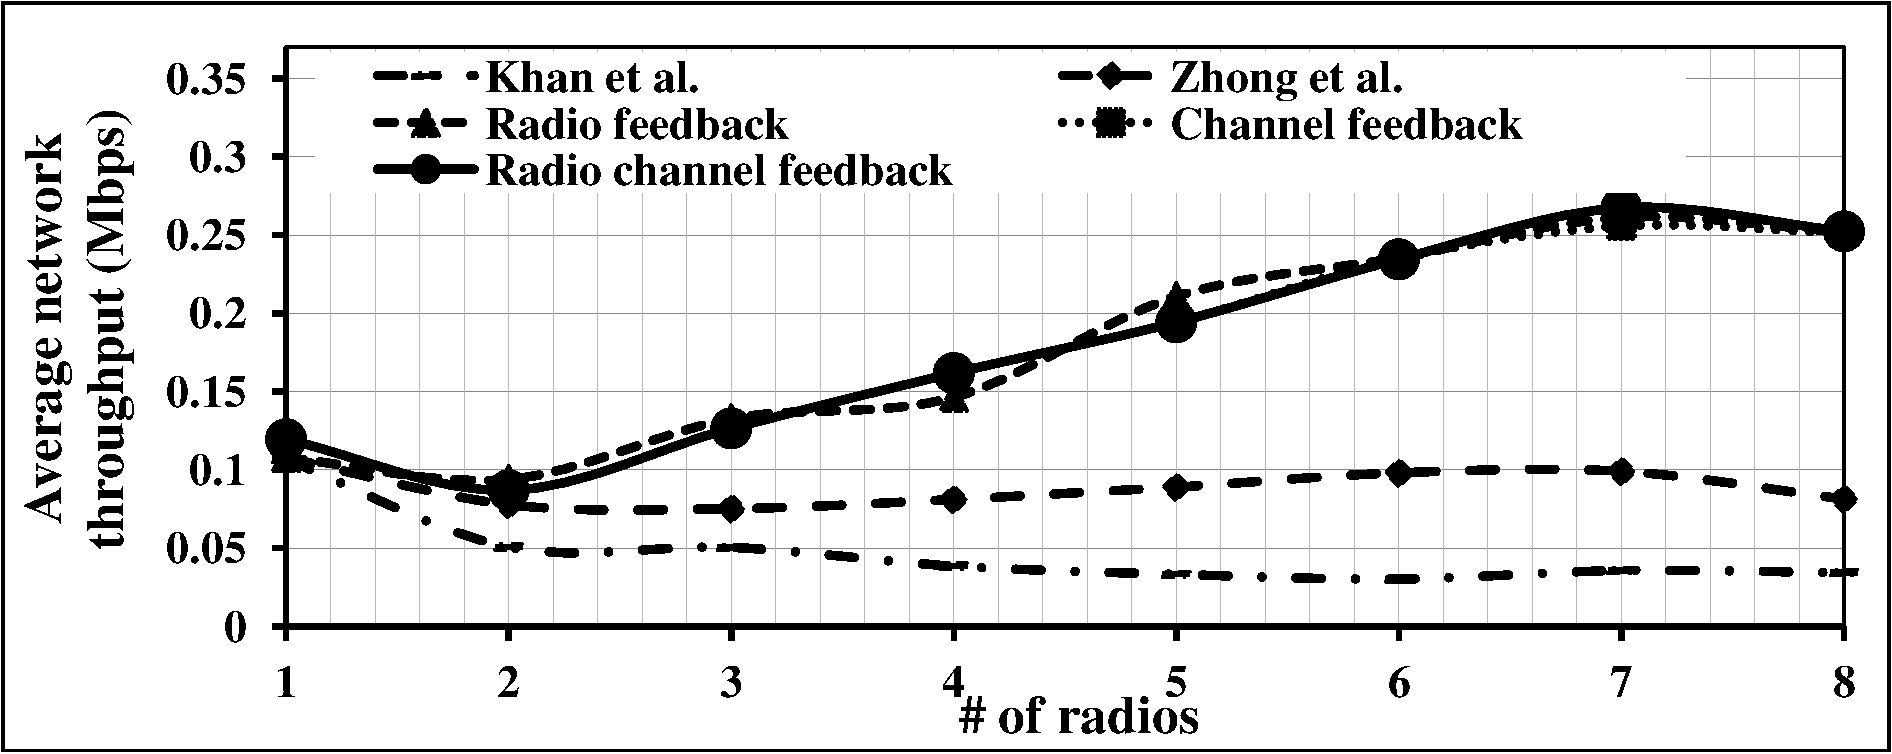
\includegraphics[width=\textwidth]{topology4/Throughput24d4}
        \caption{4Mbps application data rate}
        \label{fig:topology4T3}
    \end{subfigure}
    ~
    \begin{subfigure}[t]{0.45\textwidth}
        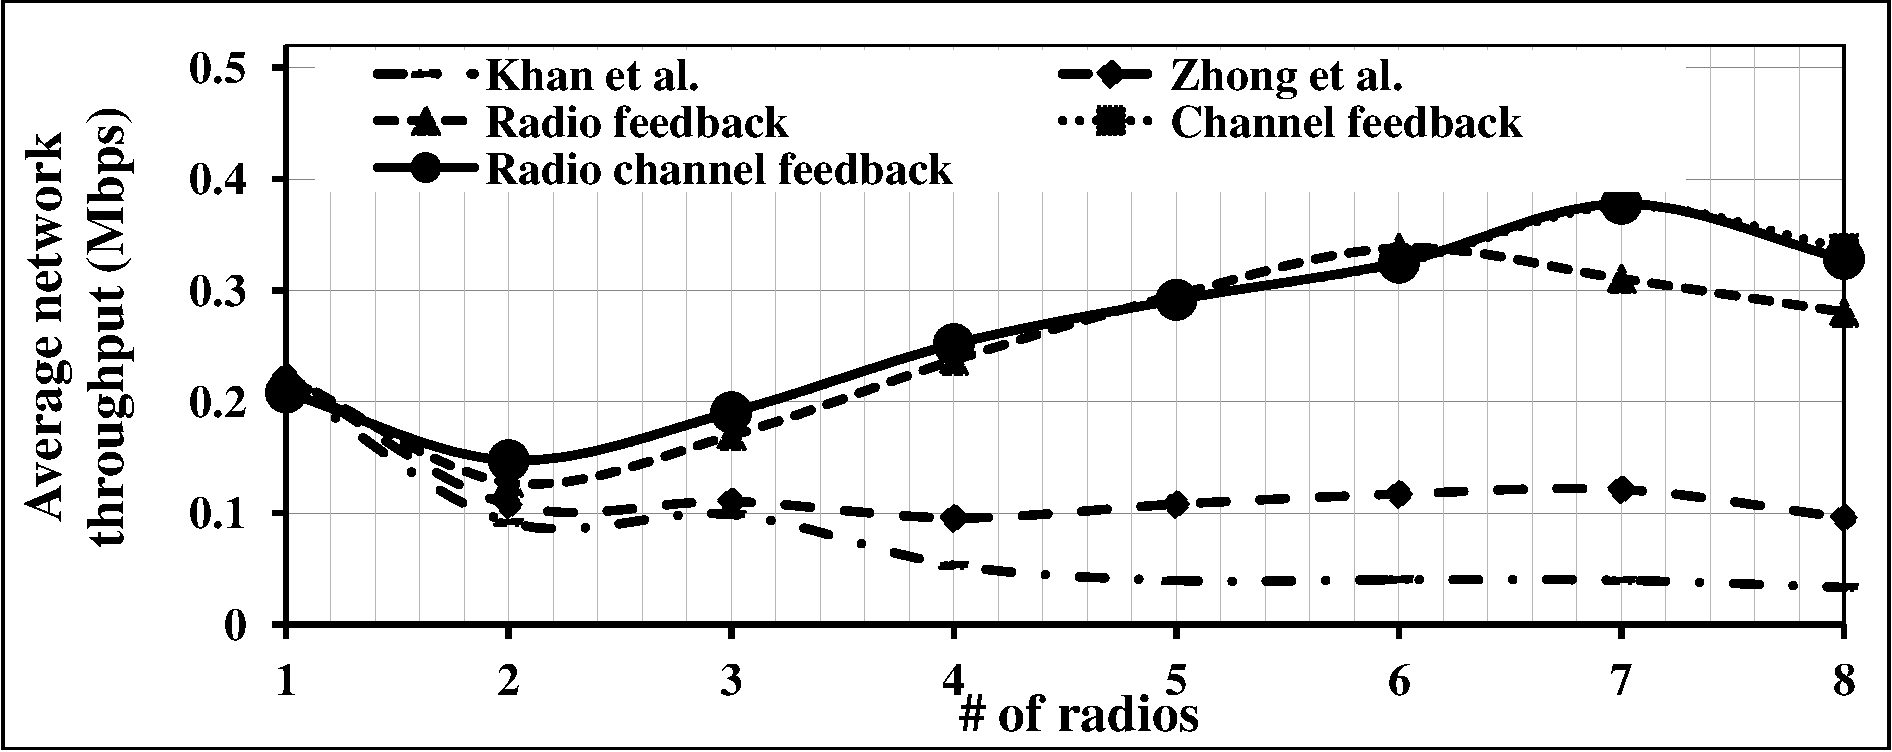
\includegraphics[width=\textwidth]{topology4/Throughput24d8}
        \caption{8Mbps application data rate}
        \label{fig:topology4T4}
    \end{subfigure}
    ~\\
    \begin{subfigure}[t]{0.45\textwidth}
        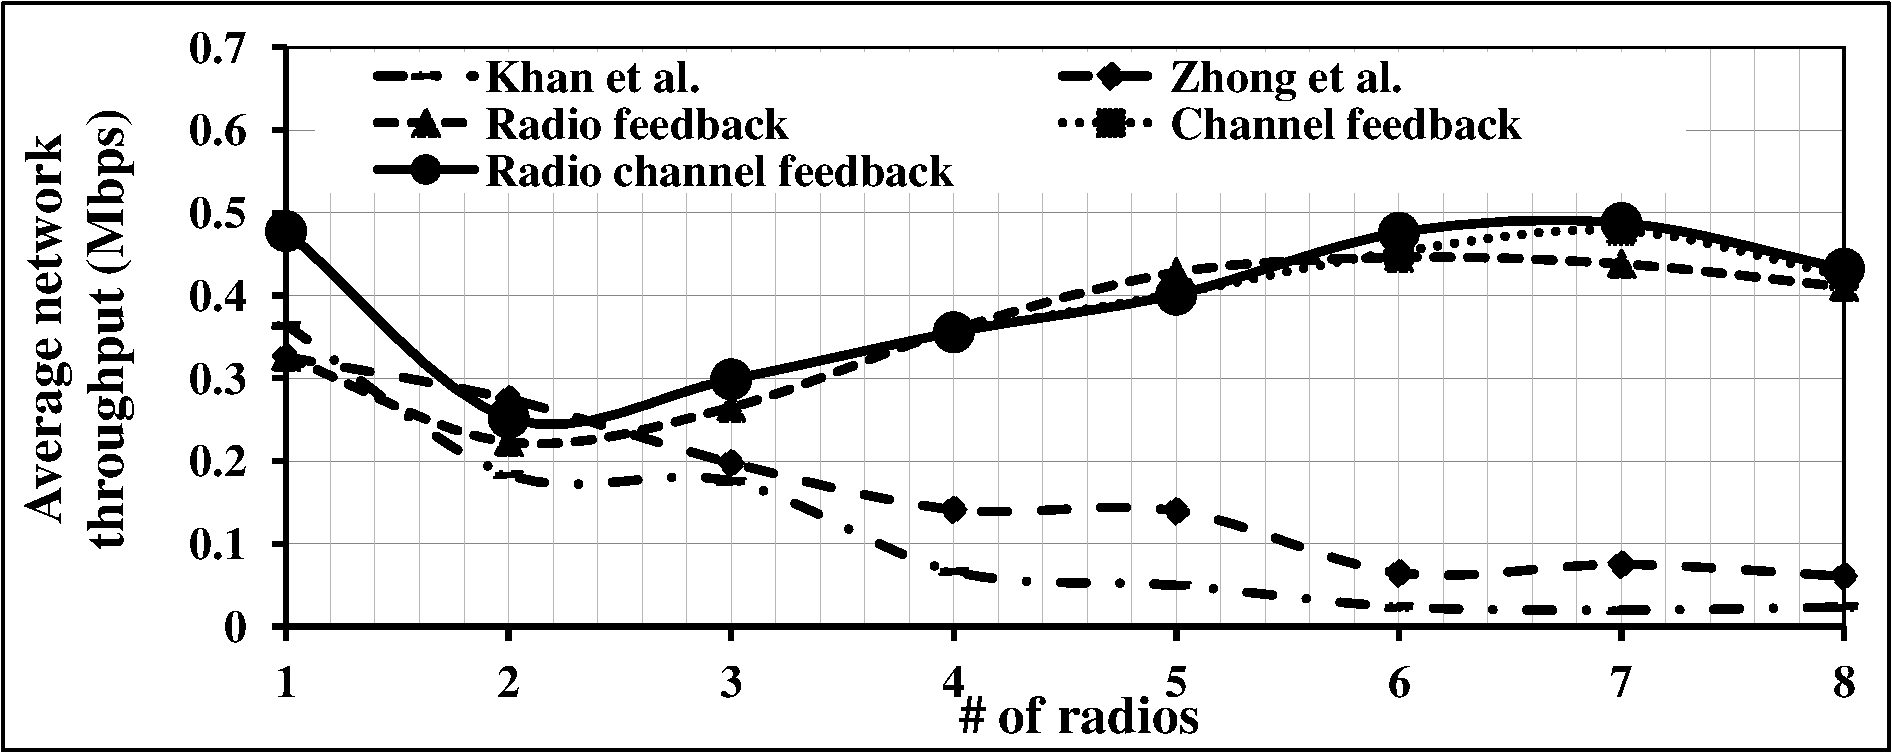
\includegraphics[width=\textwidth]{topology4/Throughput24d16}
        \caption{16Mbps application data rate}
        \label{fig:topology4T5}
    \end{subfigure}
    ~
    \begin{subfigure}[t]{0.45\textwidth}
        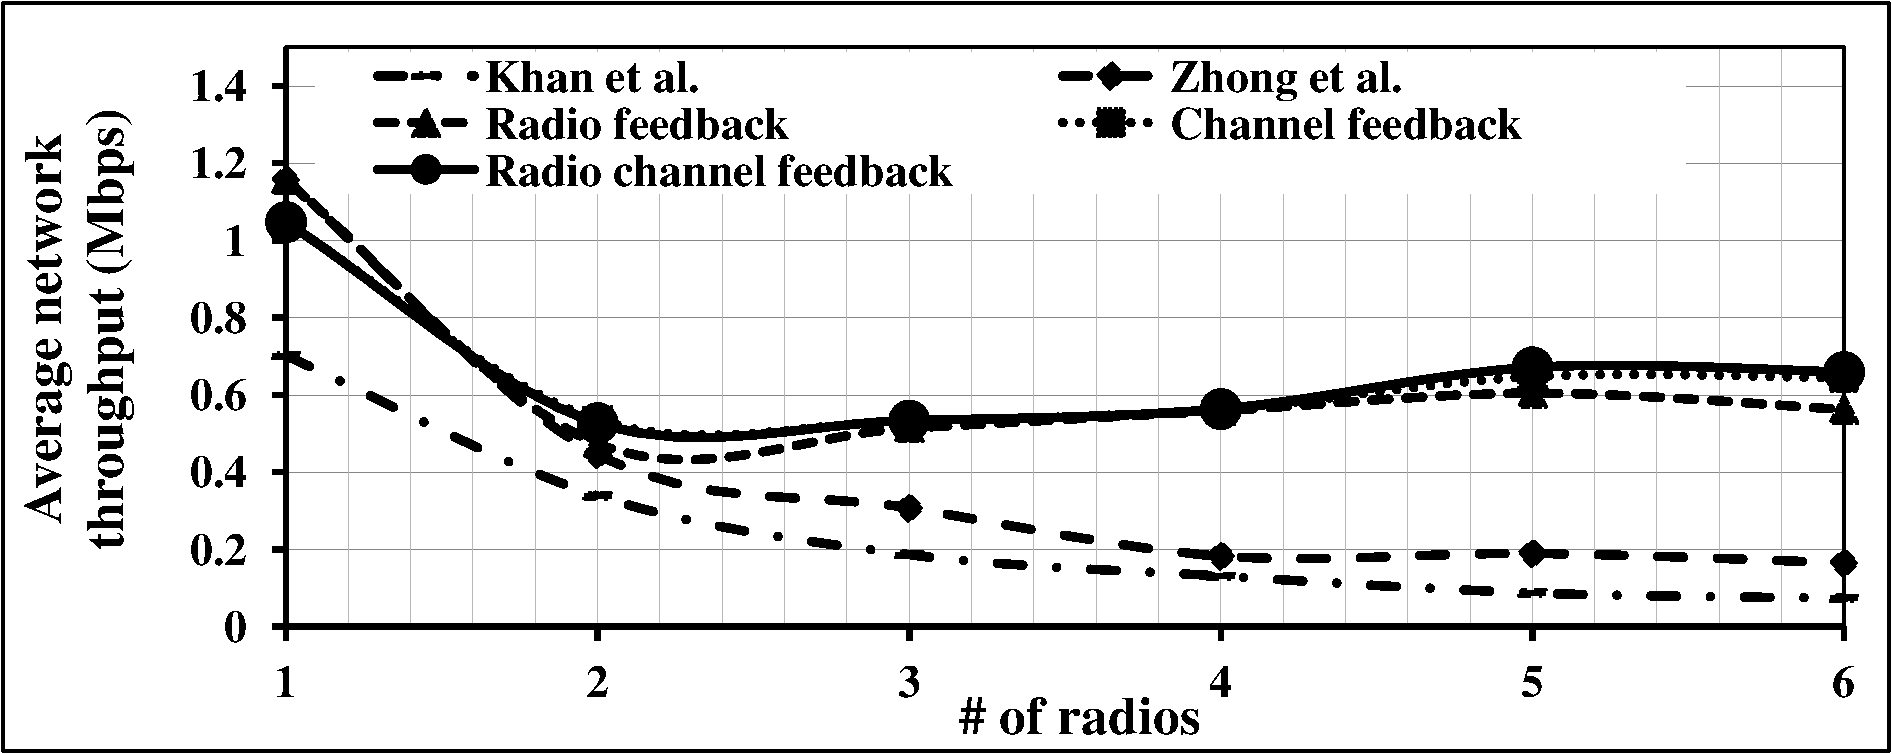
\includegraphics[width=\textwidth]{topology4/Throughput24d32}
        \caption{32Mbps application data rate}
        \label{fig:topology4T6}
    \end{subfigure}
    \caption{Average network throughput with varying number of radios for various application data rates}
    \label{fig:topology4T}
\end{figure*}

We start presenting our simulation results for a topology having 11 primary users and 24 secondary users. Here, we vary the application data rate from the source of a flow over secondary users from 1 Mbps to 32 Mbps. Figure~\ref{fig:topology4T}, \ref{fig:topology4D}, and \ref{fig:topology4P} show the performance of several variants of our proposed approach and other existing approaches.

Figure~\ref{fig:topology4T} depicts total network throughput for all the approaches in response to a variation in the number of radios for different application data rates. In most of the cases, our proposed approaches obtain significantly higher network throughput than the existing ones. Here, at lower data rates (1-8 Mbps), total network throughput increases with an increase in the number of radios. After reaching an optimal point, throughput starts degrading. At higher data rates (16 and 32 Mbps), the network throughput falls drastically from the single radio scenario and never again reaches the throughput obtained with single radio data transmission.

Figure~\ref{fig:topology4D} illustrates that the feedback-based approaches experience significantly lower end-to-end delay than that achieved with the approach proposed by Zhong et al.~\cite{zhong2014capacity}. However, delay using our proposed approach is higher than that achieved with the approach proposed by Khan et al.~\cite{khan2015towards}. Here with our proposed approach, the delay becomes almost constant with an increase in the number of radios at lower application date rates (1-4Mbps). However, at higher data rates (8-32 Mbps), the delay rises with an increase in the number of radios per SU.
\begin{figure*}[!htbp]
    \centering
    \begin{subfigure}[t]{0.45\textwidth}
        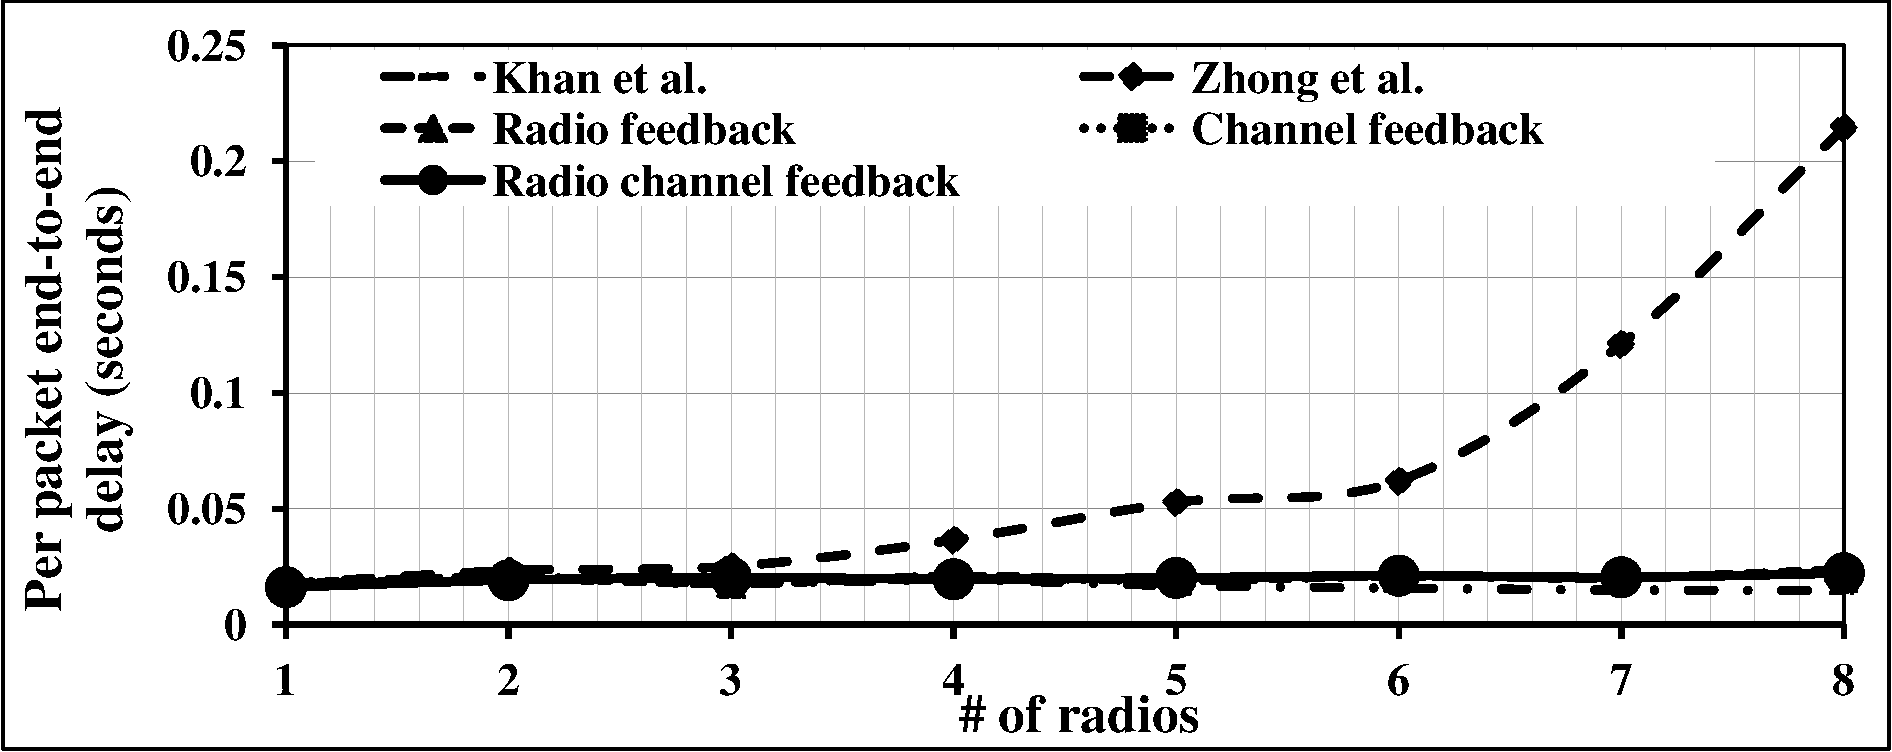
\includegraphics[width=\textwidth]{topology4/Delay24d1}
        \caption{1Mbps application data rate}
        \label{fig:topology4D1}
    \end{subfigure}
    ~
    \begin{subfigure}[t]{0.45\textwidth}
        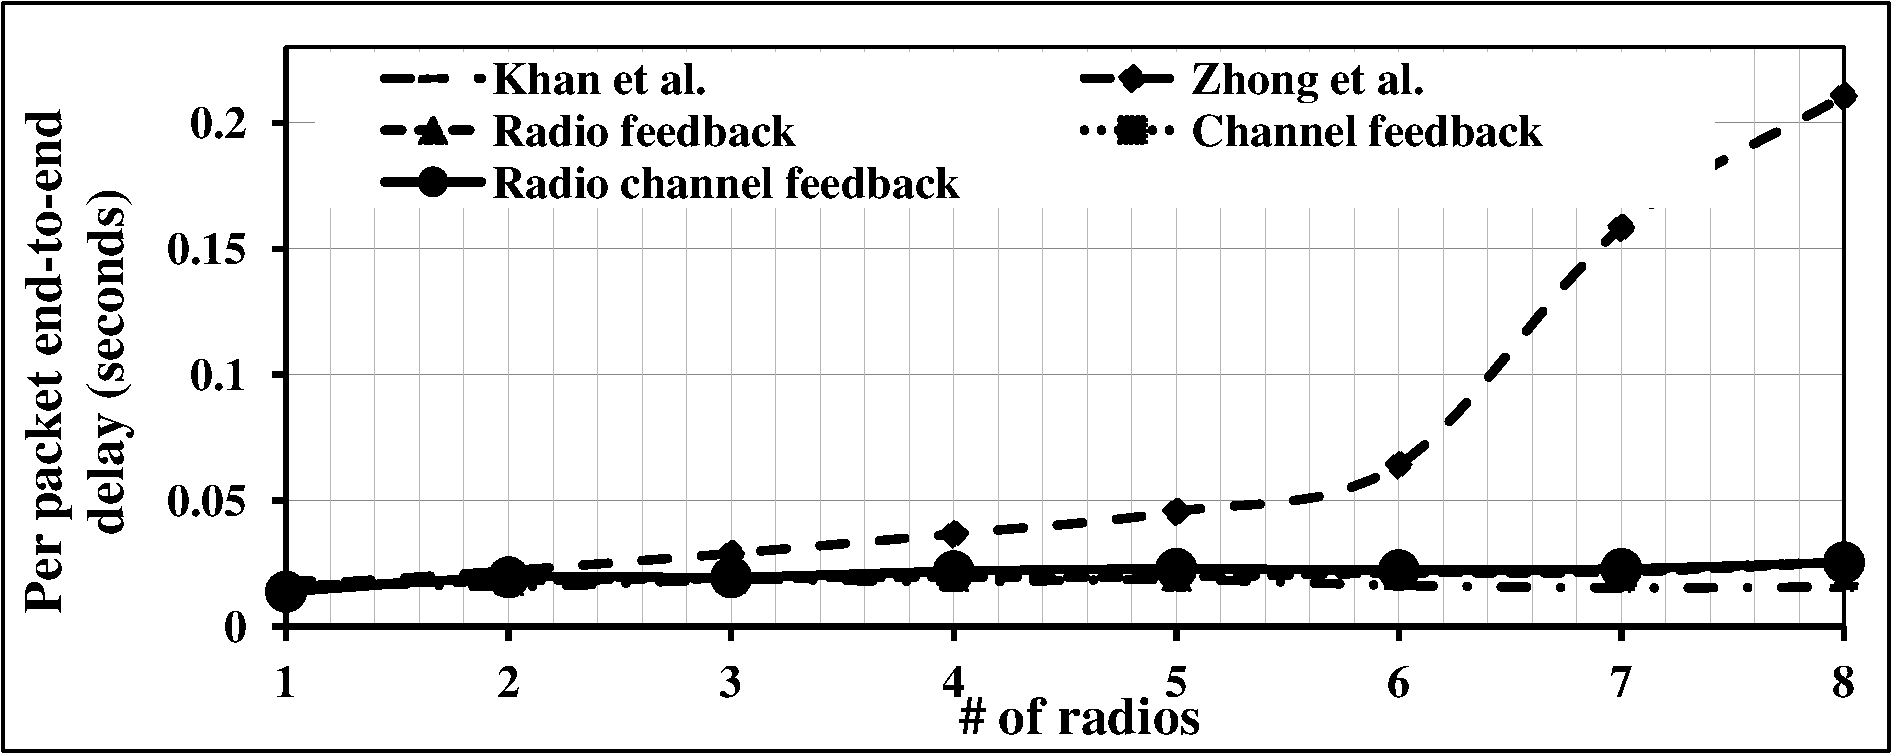
\includegraphics[width=\textwidth]{topology4/Delay24d2}
        \caption{2Mbps application data rate}
        \label{fig:topology4D2}
    \end{subfigure}
    ~\\
    \begin{subfigure}[t]{0.45\textwidth}
        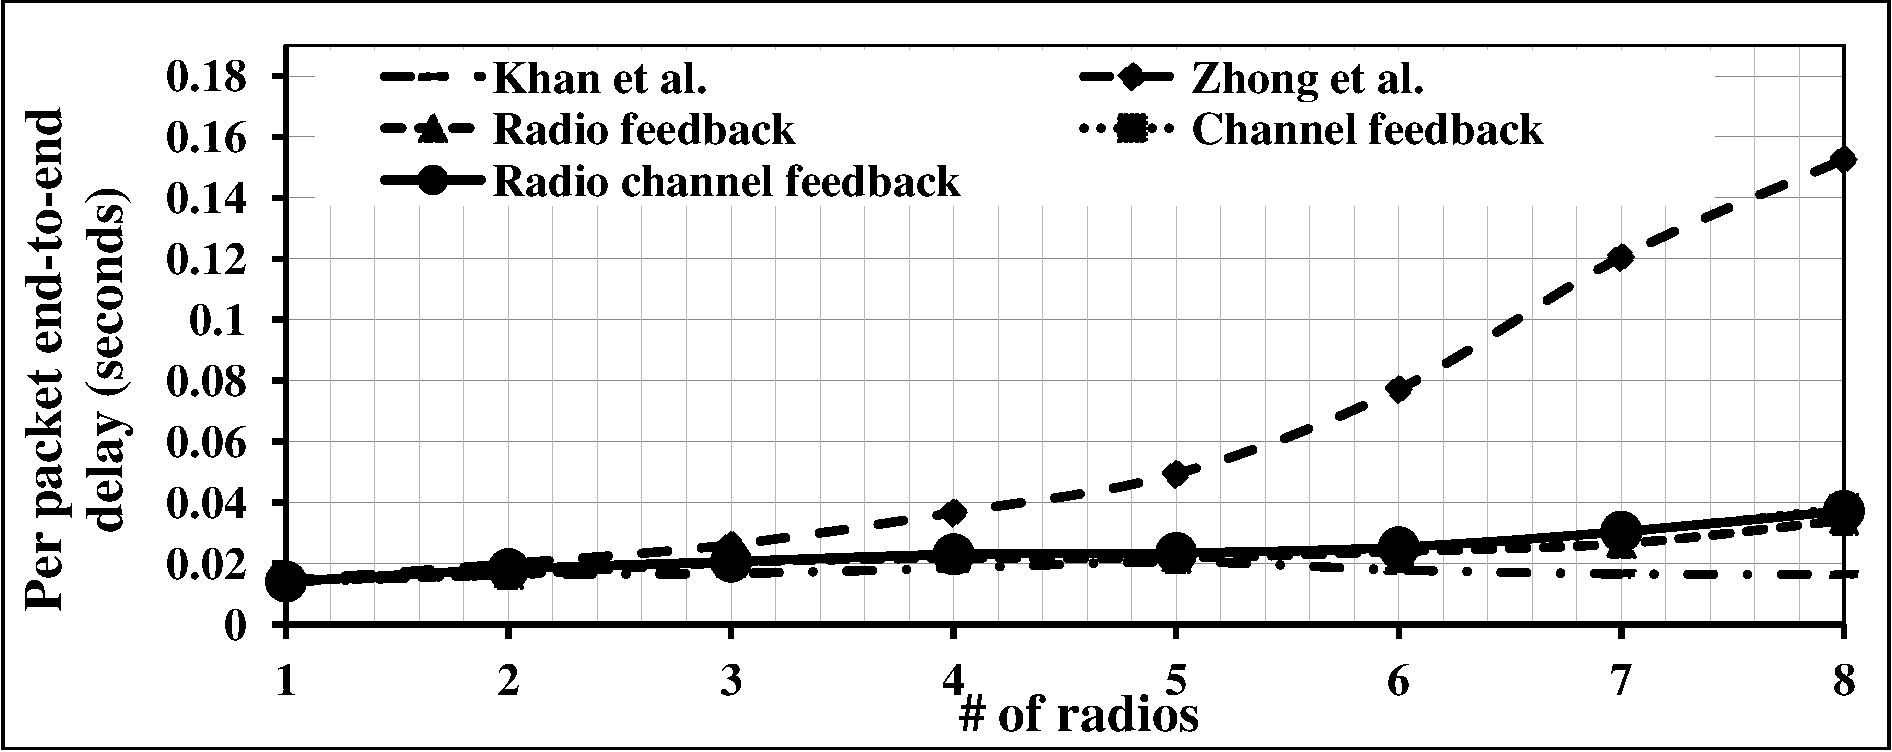
\includegraphics[width=\textwidth]{topology4/Delay24d4}
        \caption{4Mbps application data rate}
        \label{fig:topology4D3}
    \end{subfigure}
    ~
    \begin{subfigure}[t]{0.45\textwidth}
        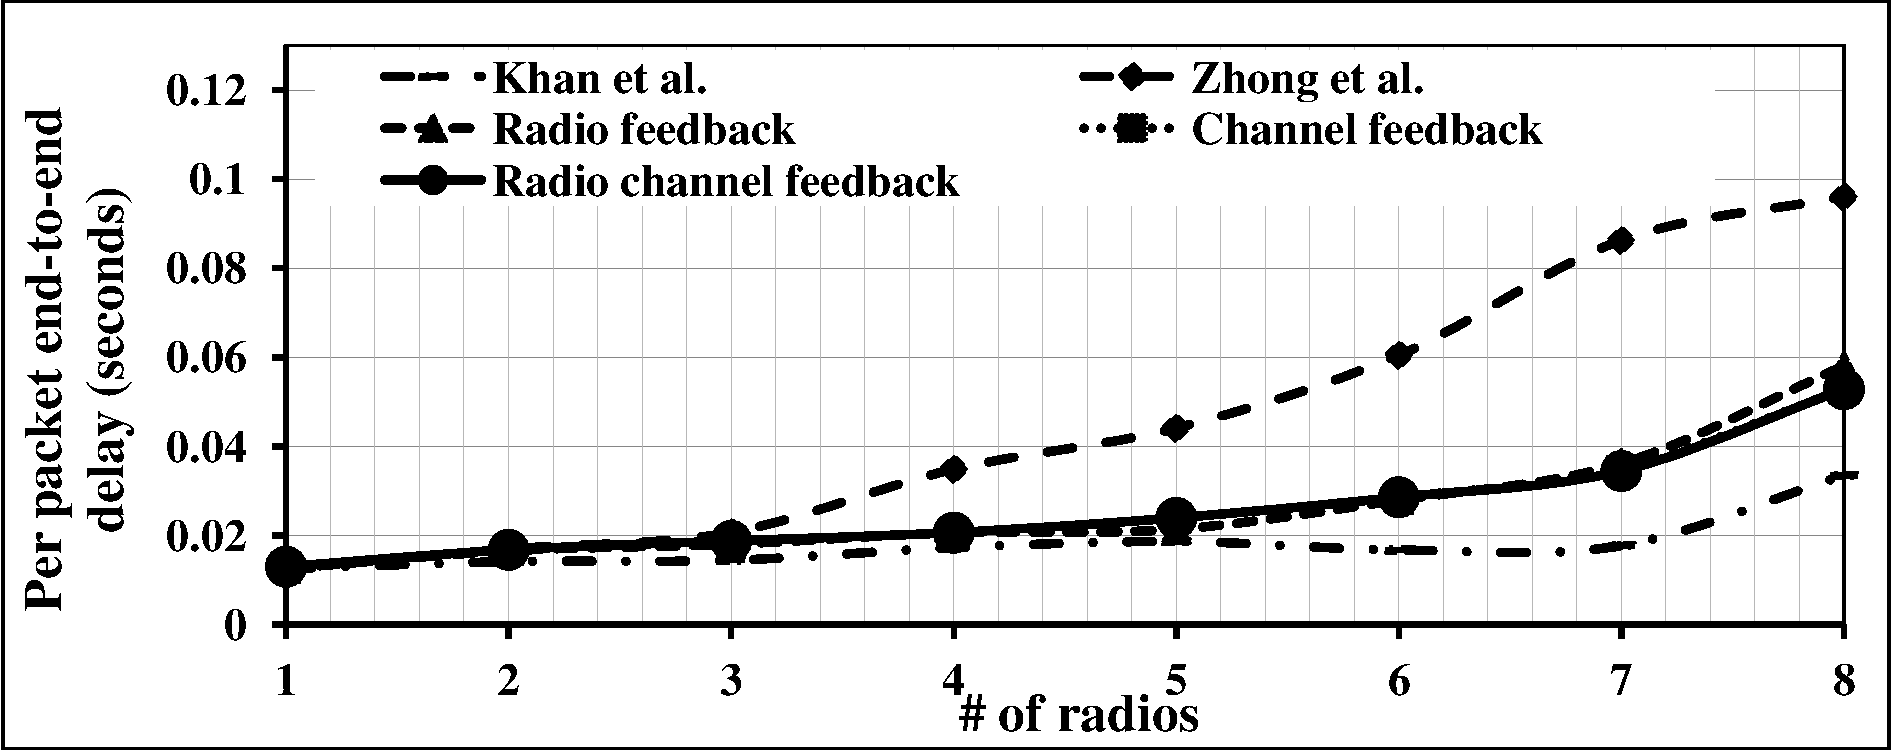
\includegraphics[width=\textwidth]{topology4/Delay24d8}
        \caption{8Mbps application data rate}
        \label{fig:topology4D4}
    \end{subfigure}
    ~\\
    \begin{subfigure}[t]{0.45\textwidth}
        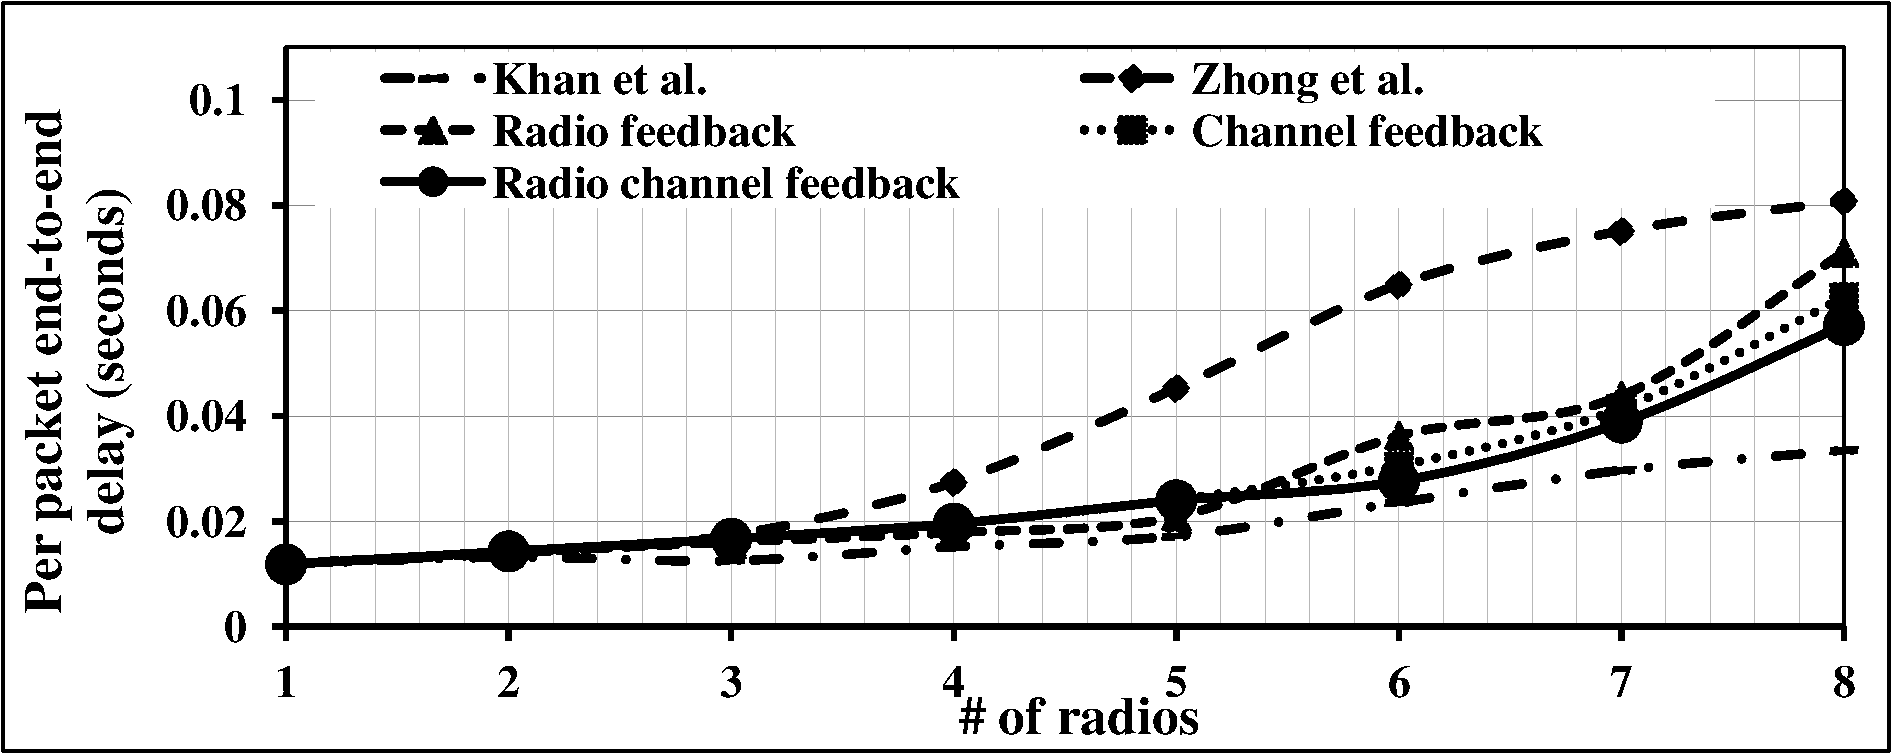
\includegraphics[width=\textwidth]{topology4/Delay24d16}
        \caption{16Mbps application data rate}
        \label{fig:topology4D5}
    \end{subfigure}
    ~
    \begin{subfigure}[t]{0.45\textwidth}
        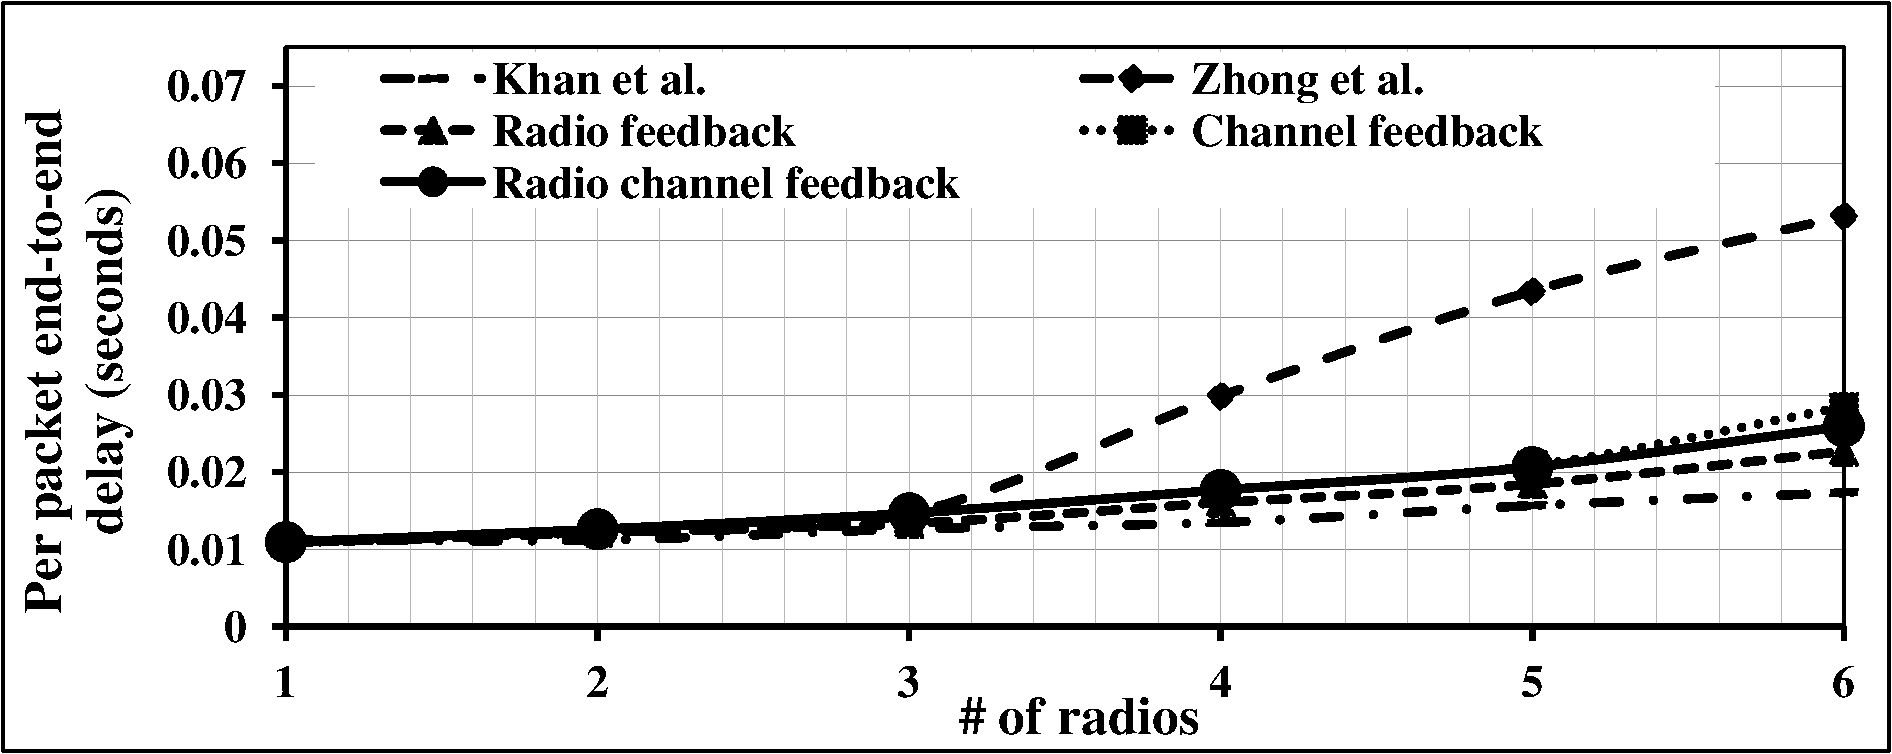
\includegraphics[width=\textwidth]{topology4/Delay24d32}
        \caption{32Mbps application data rate}
        \label{fig:topology4D6}
    \end{subfigure}
    \caption{Average end-to-end delay with varying number of radios for various application data rates}
    \label{fig:topology4D}
\end{figure*}


Figure~\ref{fig:topology4P} compares the average packet drop ratio of our proposed approaches against that of the existing approaches.  As illustrated in Figure~\ref{fig:topology4P}, the feedback-based approach achieves significantly lower packet drop ratios than all the existing ones. The feedback-based approach is also able to reduce the packet drop ratio significantly at lower data rates (1-8 Mbps) with the exploitation of multiple radios. However, at higher application data rates (16 and 32 Mbps), most of the packets get dropped resulting in high drop ratios. This explains why the network throughput at higher data rate does not improve even after the introduction of multiple data transmission radios.

Figure~\ref{fig:topology4PD} shows the application layer packet delivery ratio of our proposed approaches against that of the existing approaches. Due to the efficient exploitation of multiple radios, our proposed approaches obtain significantly better packet delivery ratio than that achieved with the existing appraoches.

Table~\ref{tab:topology4RadioImprovement}, \ref{tab:topology4ChannelImprovement}, and \ref{tab:topology4RadioChannelImprovement} summarize average performance improvement using feedback-based approaches in comparison to the approaches proposed by Khan et al.,~\cite{khan2015towards} and Zhong et al.~\cite{zhong2014capacity}. The tables shows that the proposed approach outperforms the existing approaches in terms of all the performance metrics except end-to-end delay. In terms of total network throughput, the proposed approach obtains an average of 51\% improvement over the two existing approaches. Moreover, the proposed approach decreases packet drop ratio on an average 35\% and increases application layer packet delivery ratio on an average 32\% compared to existing approaches. Even though, the feedback-based approach experiences the higher delay in some cases, in average, the delay is improved by 13\% on an average.
\begin{landscape}
\begin{figure*}[!htbp]
    \centering
    \begin{subfigure}[t]{0.625\textwidth}
        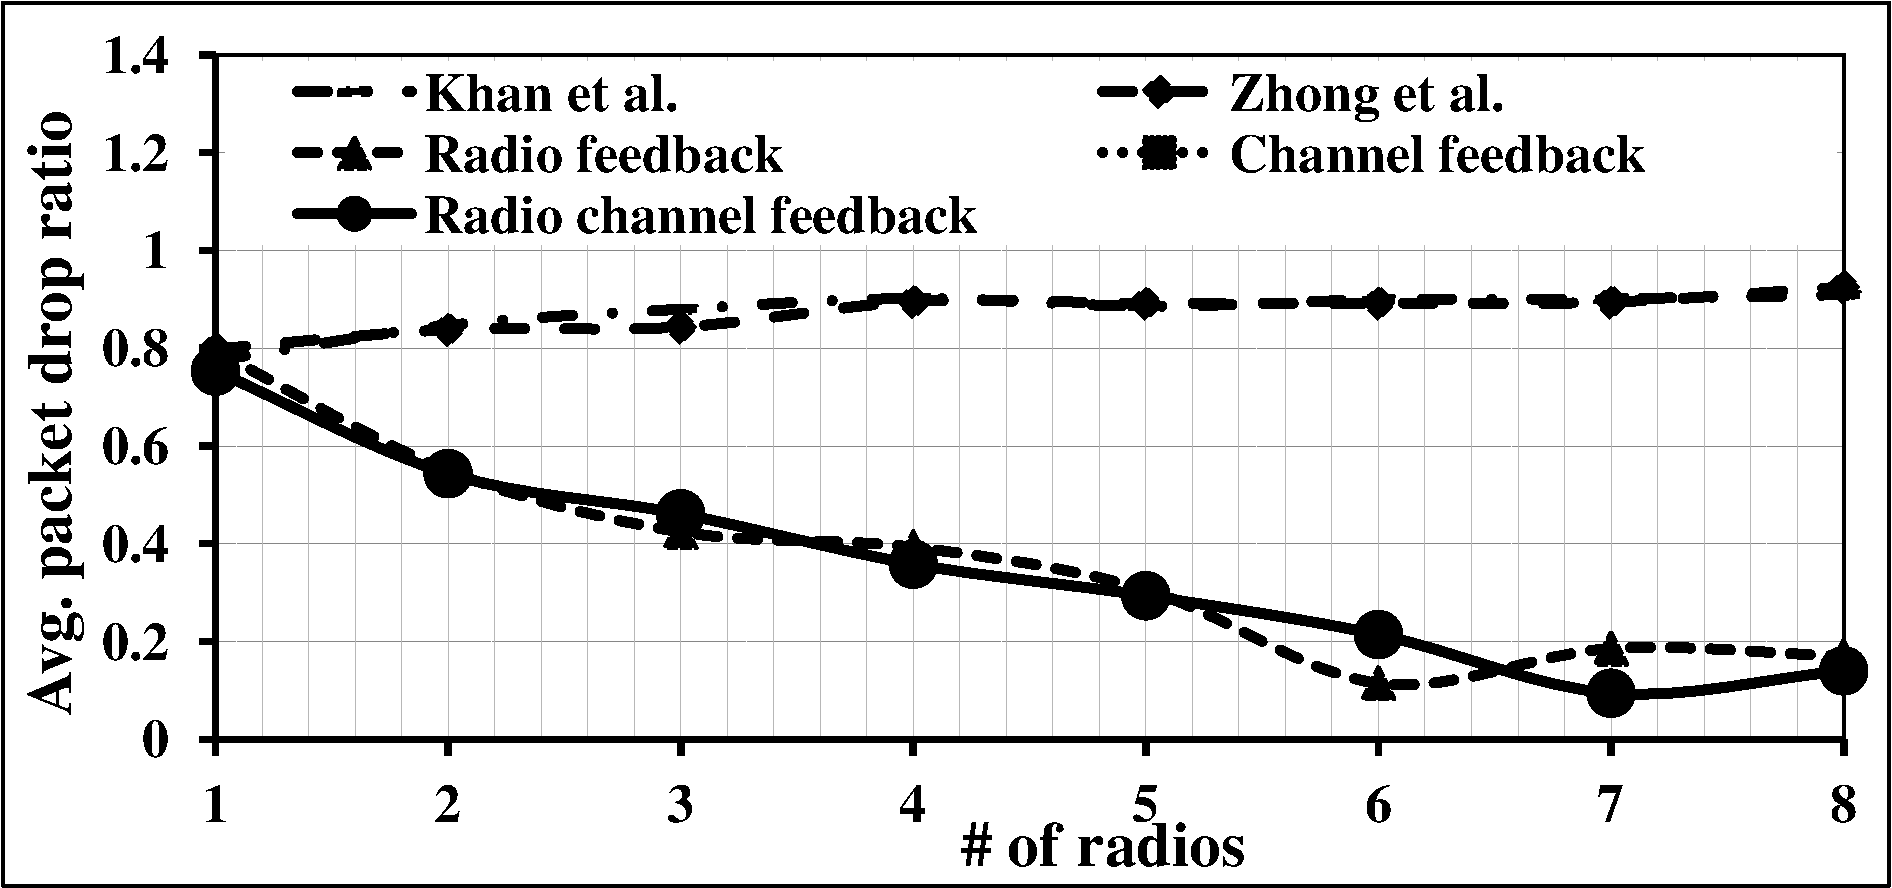
\includegraphics[width=\textwidth]{topology4/PacketDropRatio24d1}
        \caption{1Mbps application data rate}
        \label{fig:topology4P1}
    \end{subfigure}
    ~
    \begin{subfigure}[t]{0.625\textwidth}
        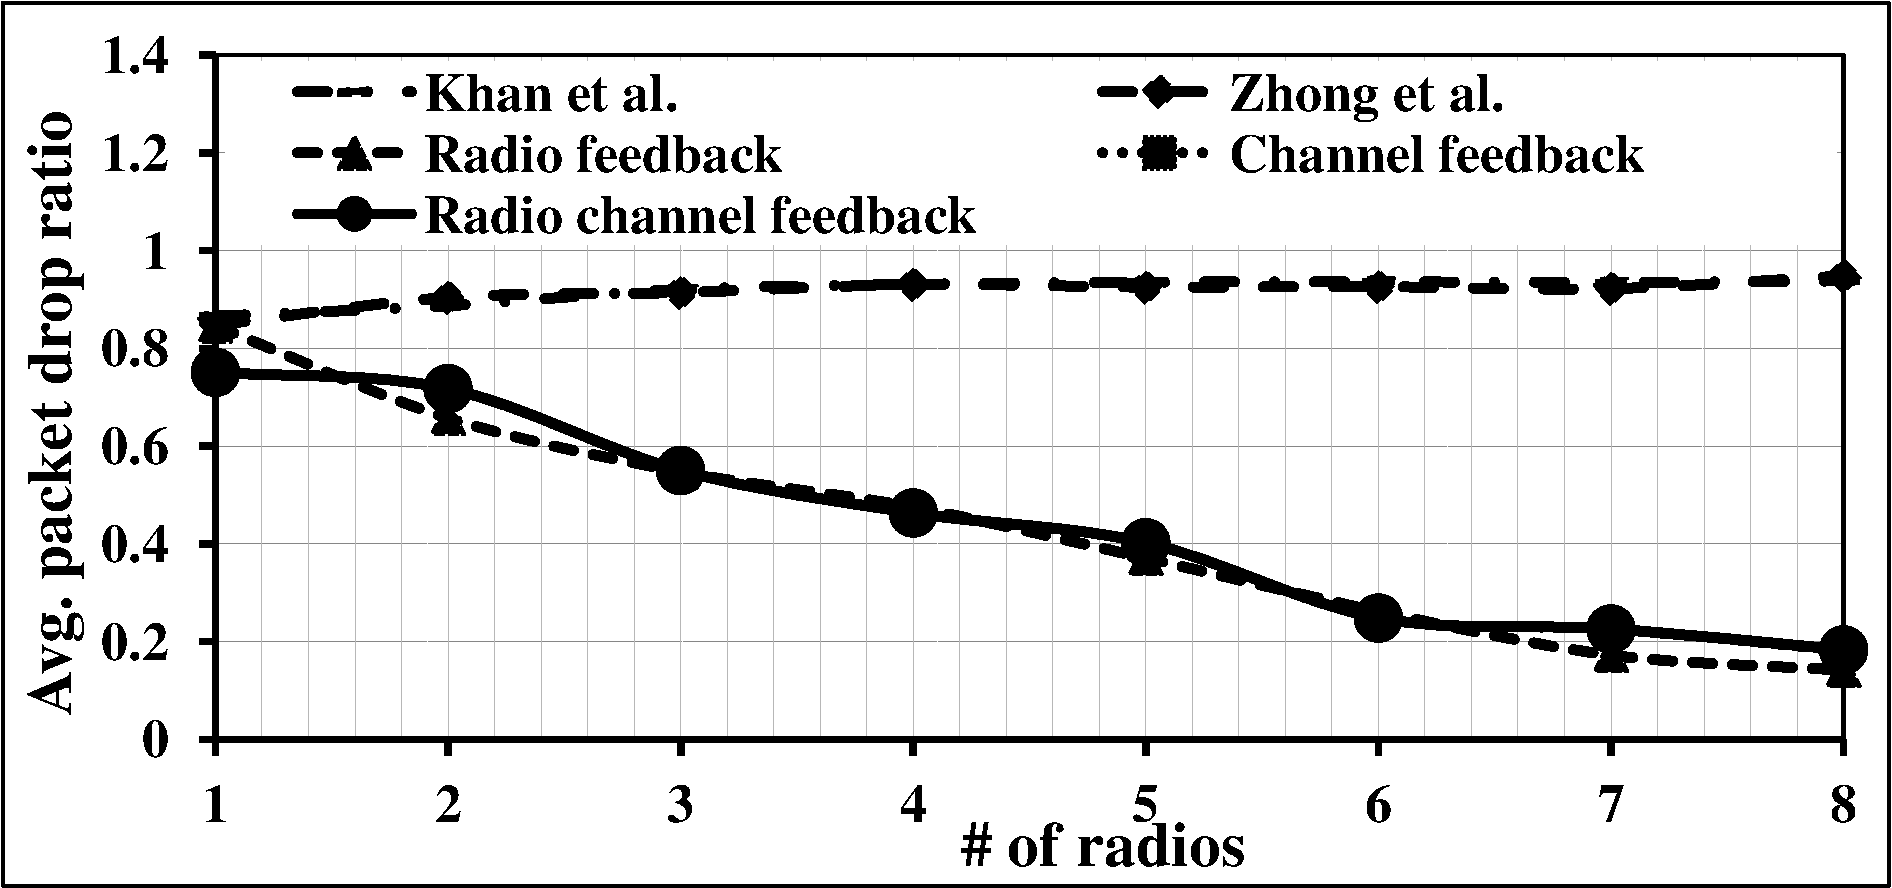
\includegraphics[width=\textwidth]{topology4/PacketDropRatio24d2}
        \caption{2Mbps application data rate}
        \label{fig:topology4P2}
    \end{subfigure}
    ~\\
    \begin{subfigure}[t]{0.625\textwidth}
        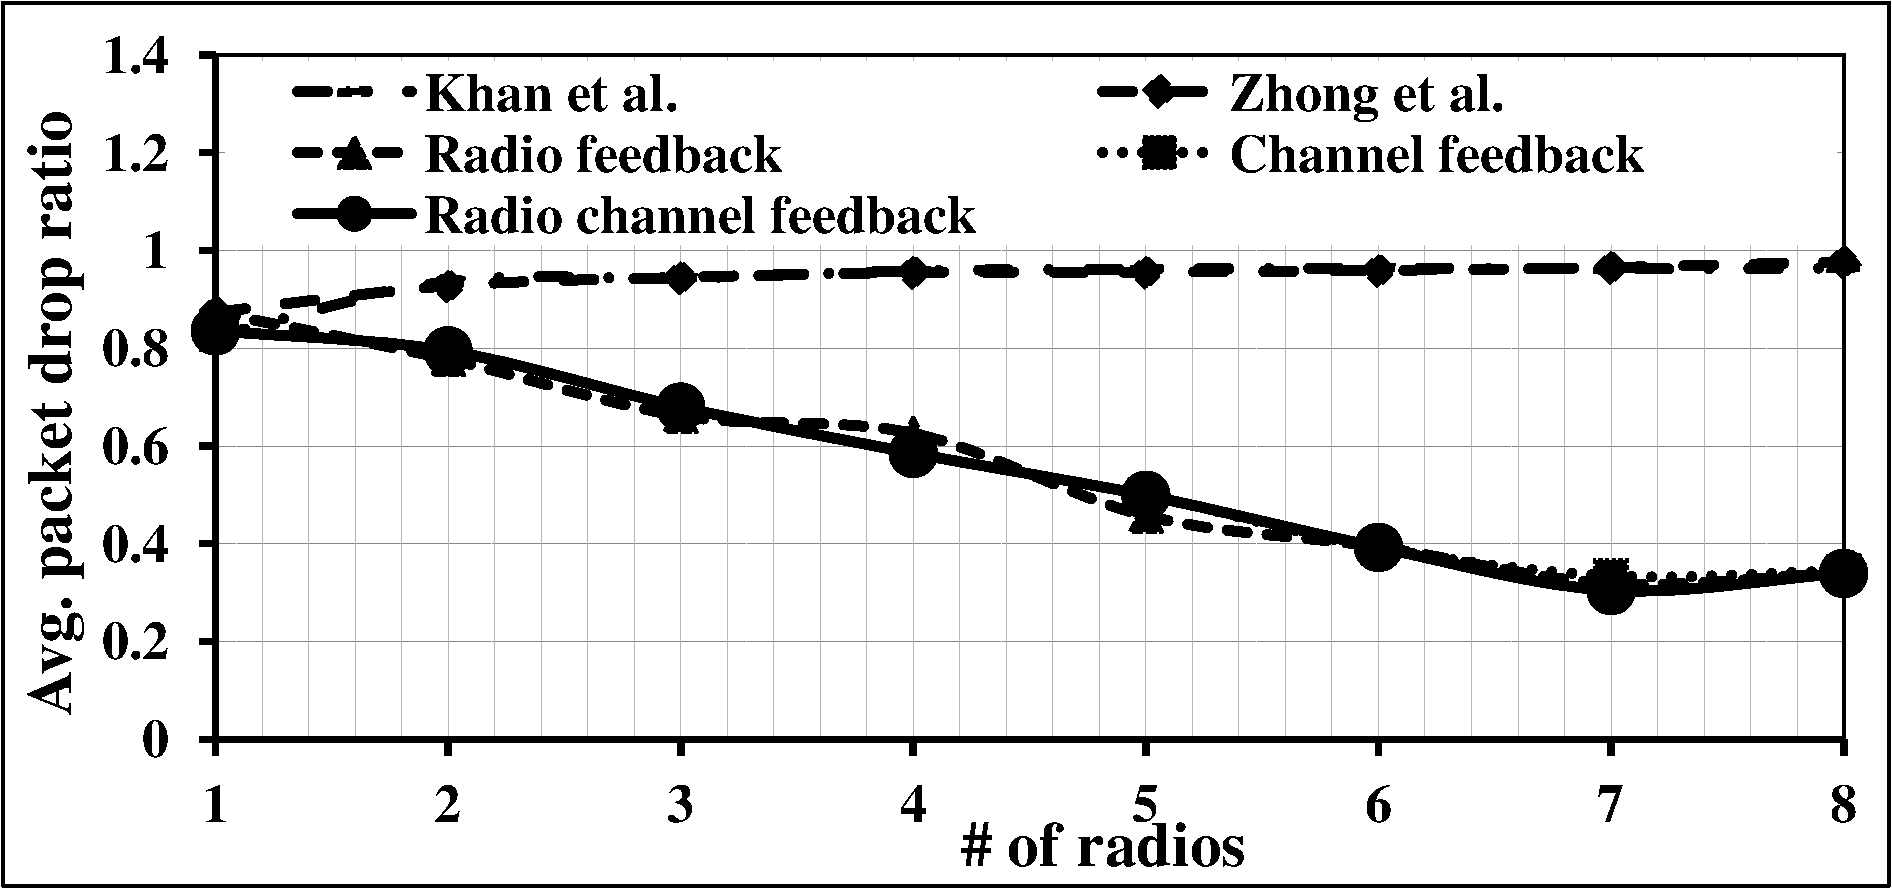
\includegraphics[width=\textwidth]{topology4/PacketDropRatio24d4}
        \caption{4Mbps application data rate}
        \label{fig:topology4P3}
    \end{subfigure}
    ~
    \begin{subfigure}[t]{0.625\textwidth}
        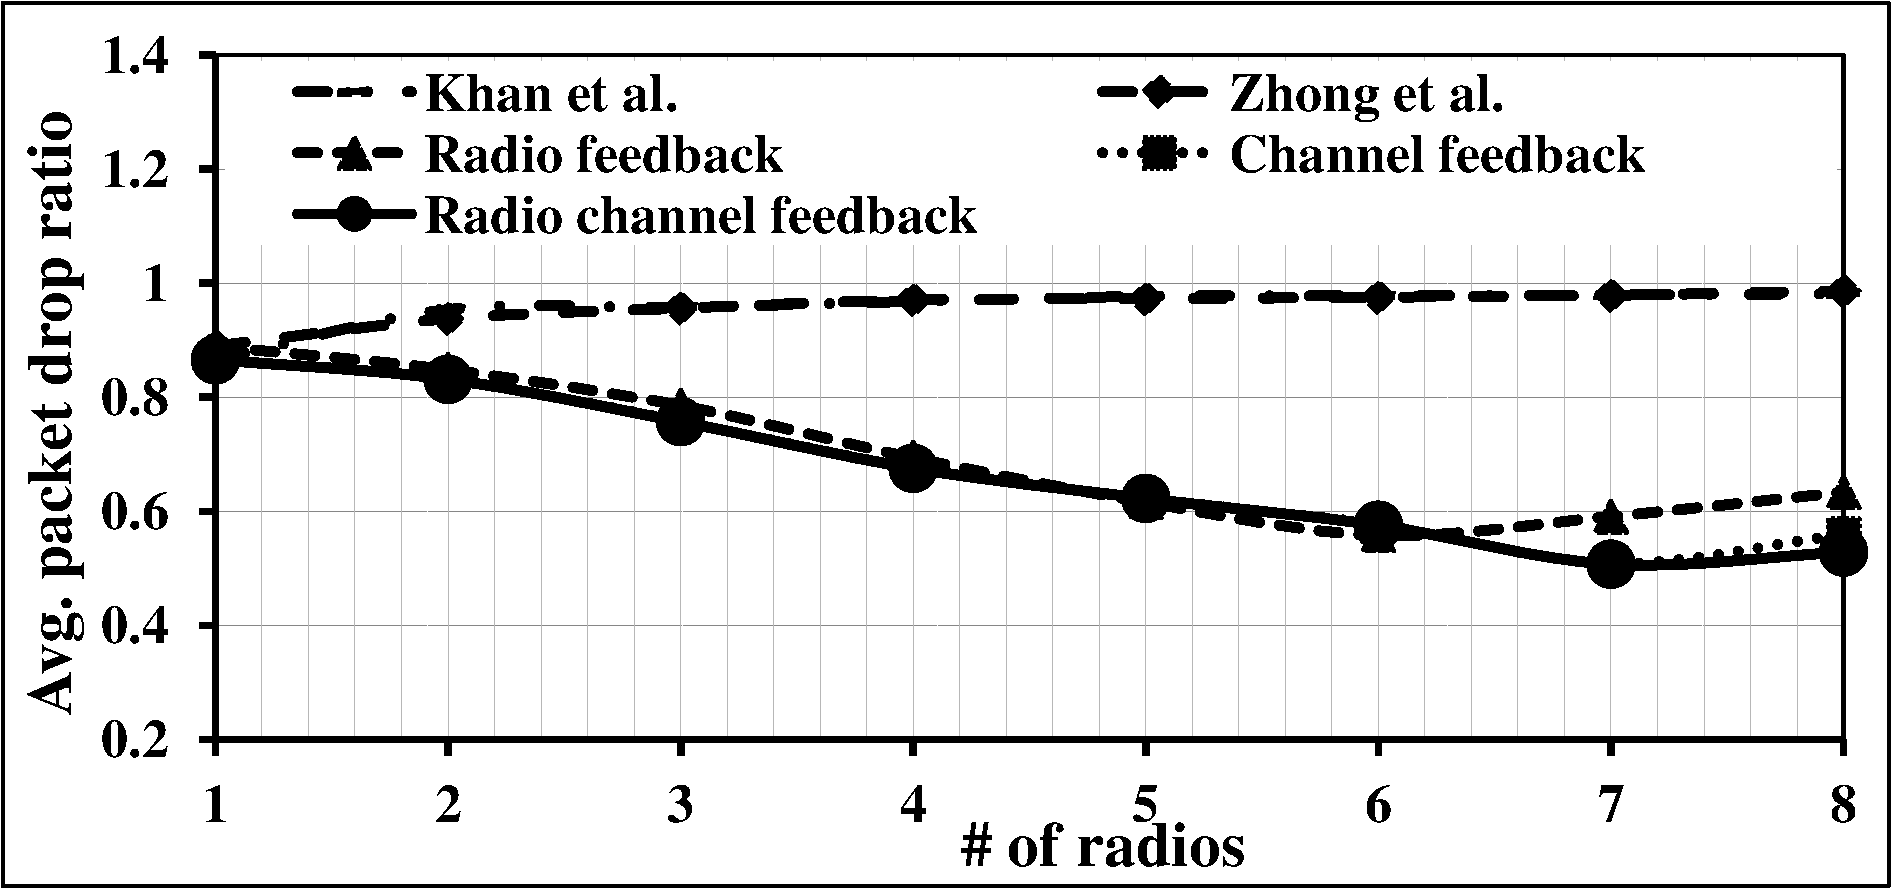
\includegraphics[width=\textwidth]{topology4/PacketDropRatio24d8}
        \caption{8Mbps application data rate}
        \label{fig:topology4P4}
    \end{subfigure}
    ~\\
    \begin{subfigure}[t]{0.625\textwidth}
        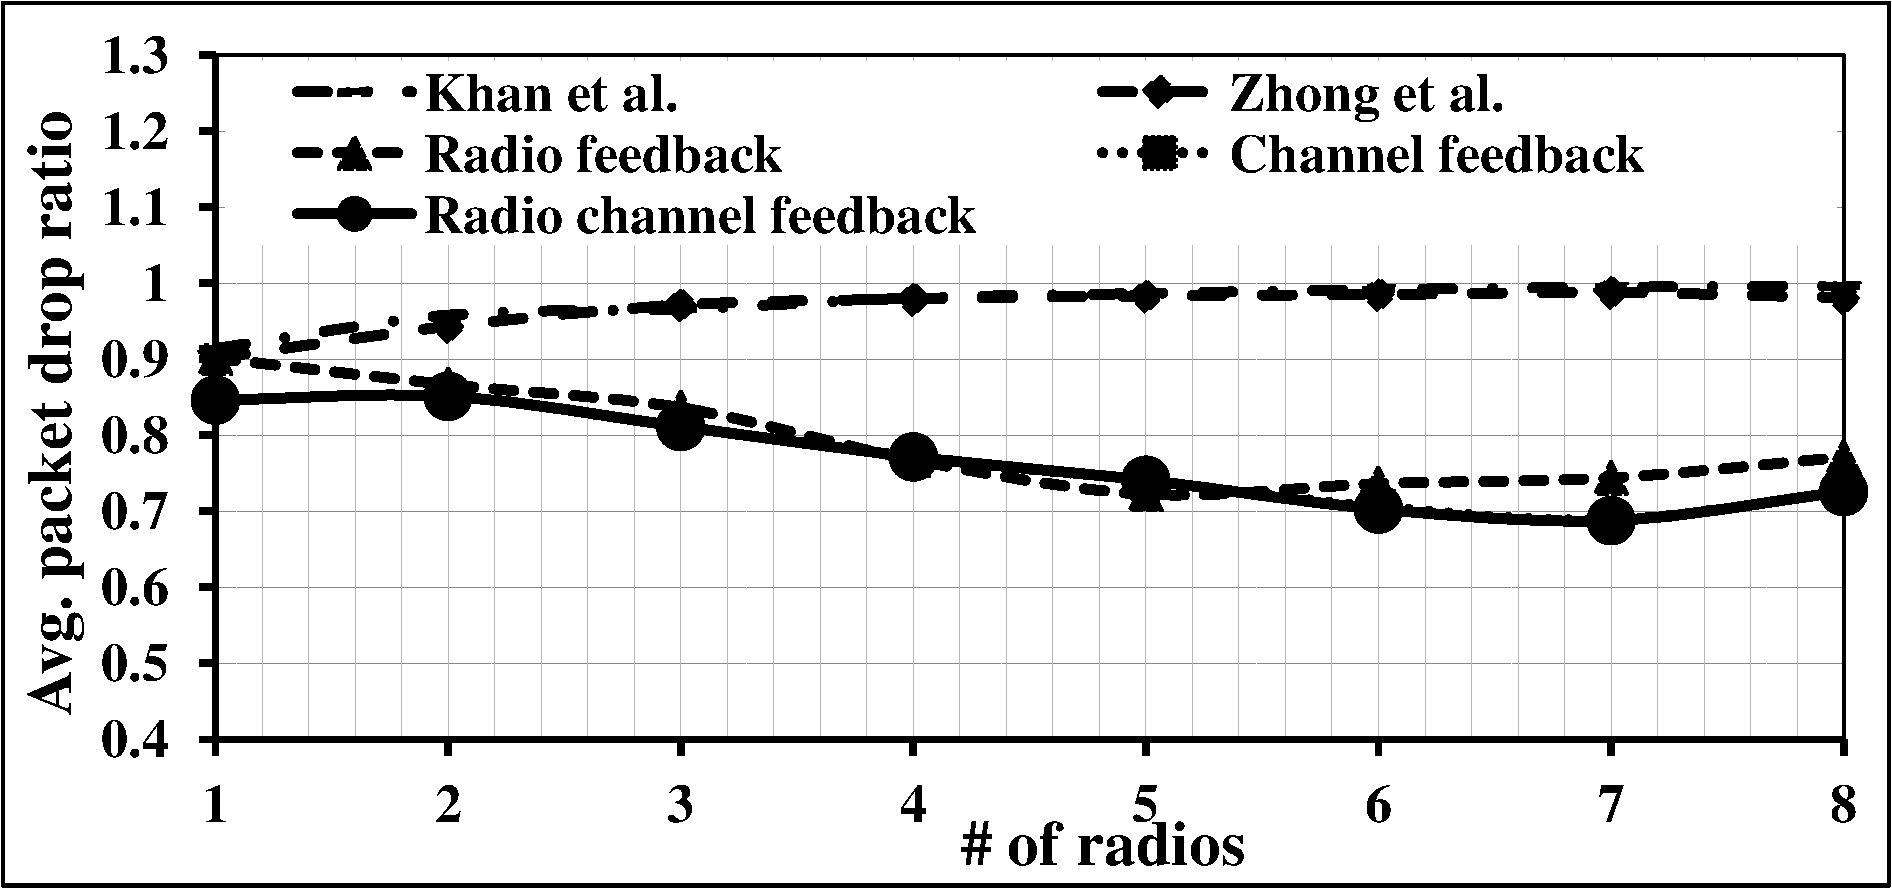
\includegraphics[width=\textwidth]{topology4/PacketDropRatio24d16}
        \caption{16Mbps application data rate}
        \label{fig:topology4P5}
    \end{subfigure}
    ~
    \begin{subfigure}[t]{0.625\textwidth}
        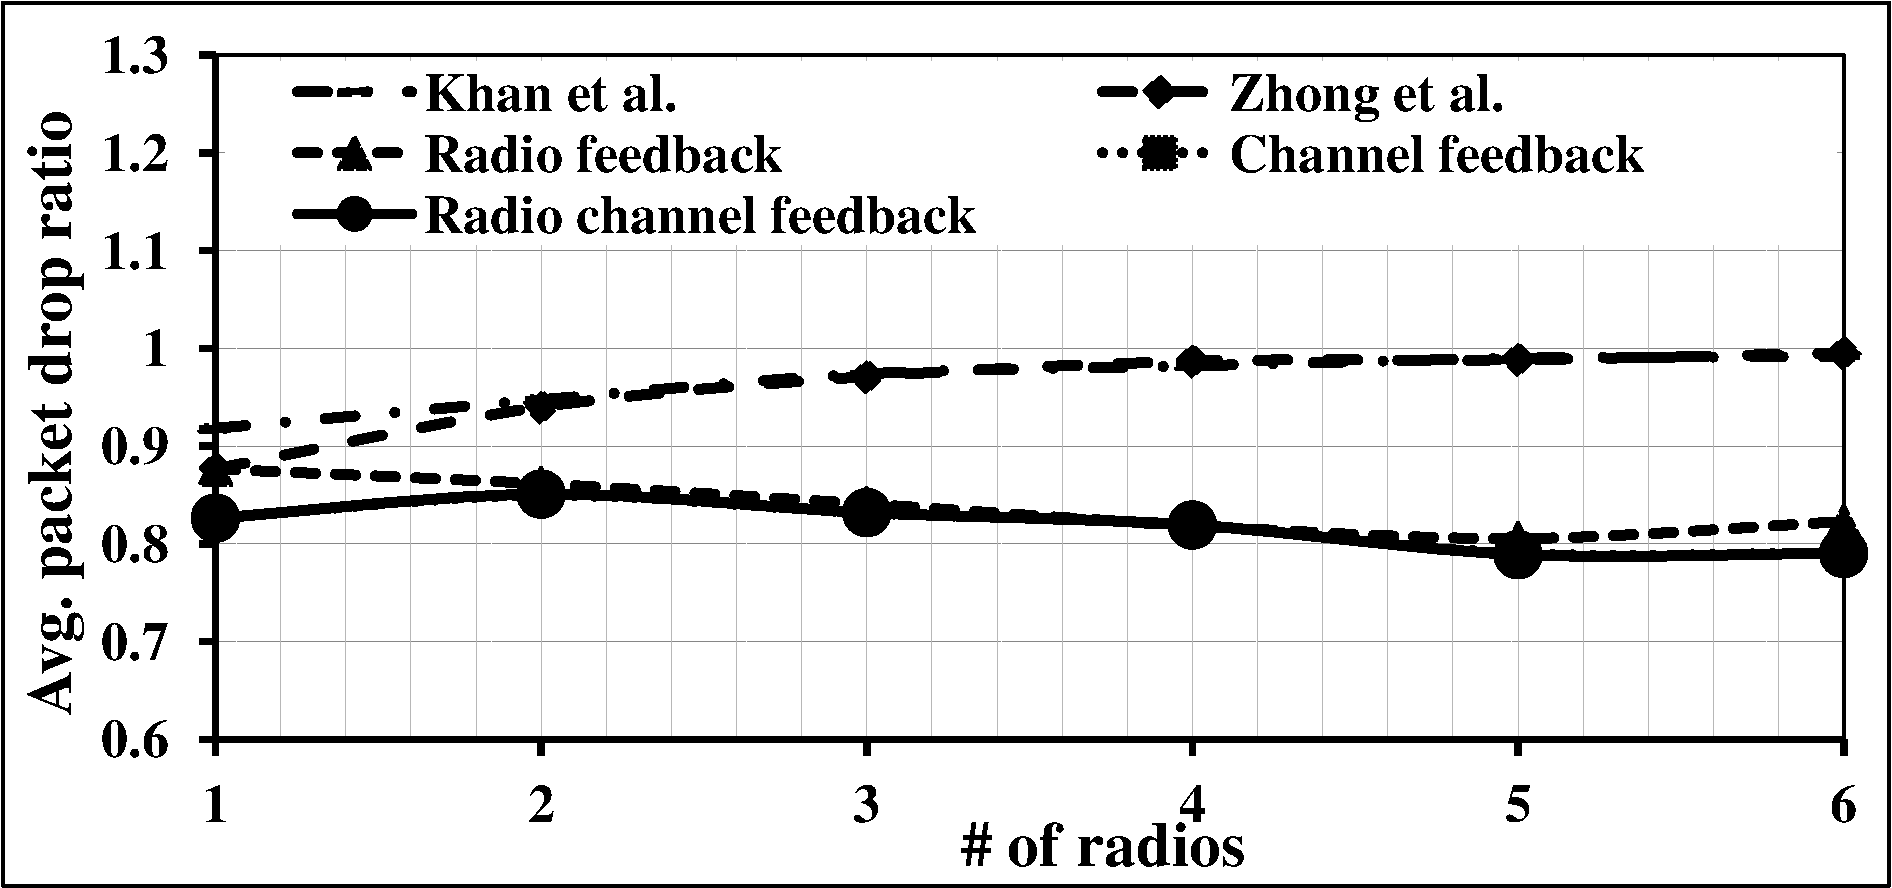
\includegraphics[width=\textwidth]{topology4/PacketDropRatio24d32}
        \caption{32Mbps application data rate}
        \label{fig:topology4P6}
    \end{subfigure}
    \caption{Average packet drop ratio with varying number of radios for various application data rates}
    \label{fig:topology4P}
\end{figure*}
\end{landscape}

\begin{figure*}[!htbp]
    \centering
    \begin{subfigure}[t]{0.45\textwidth}
        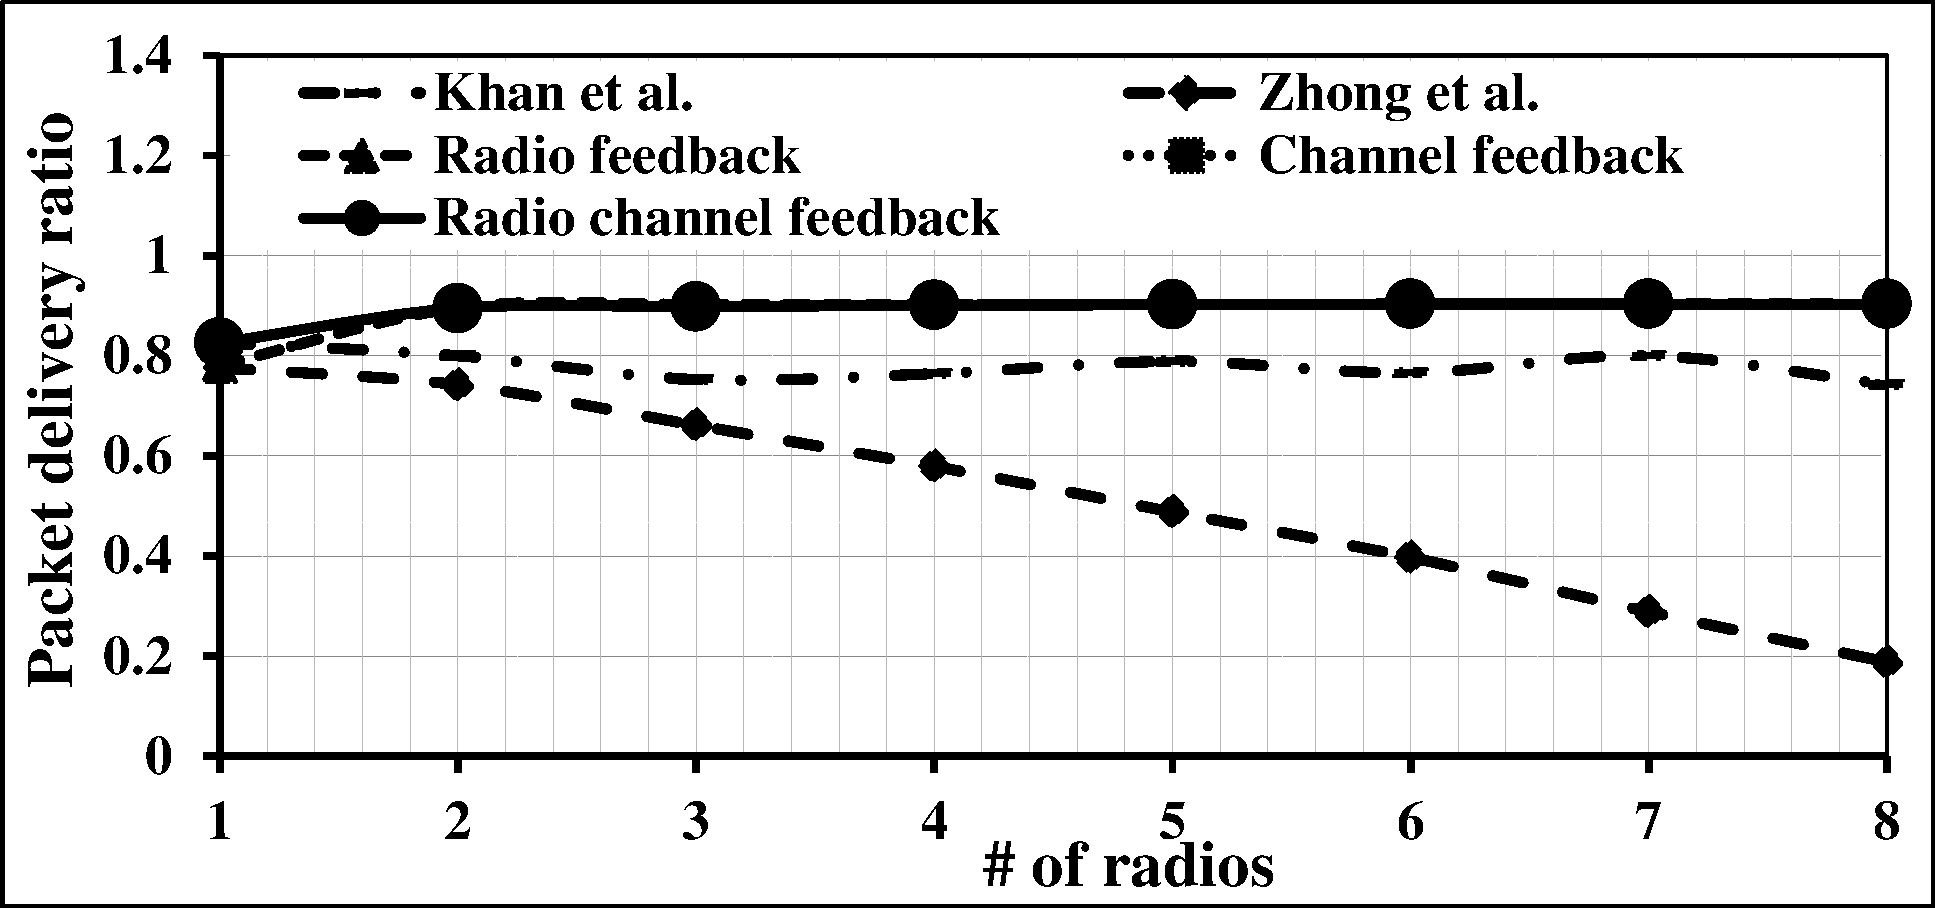
\includegraphics[width=\textwidth]{topology4/DeliveryRatio24d1}
        \caption{1Mbps application data rate}
        \label{fig:topology4PD1}
    \end{subfigure}
    ~
    \begin{subfigure}[t]{0.45\textwidth}
        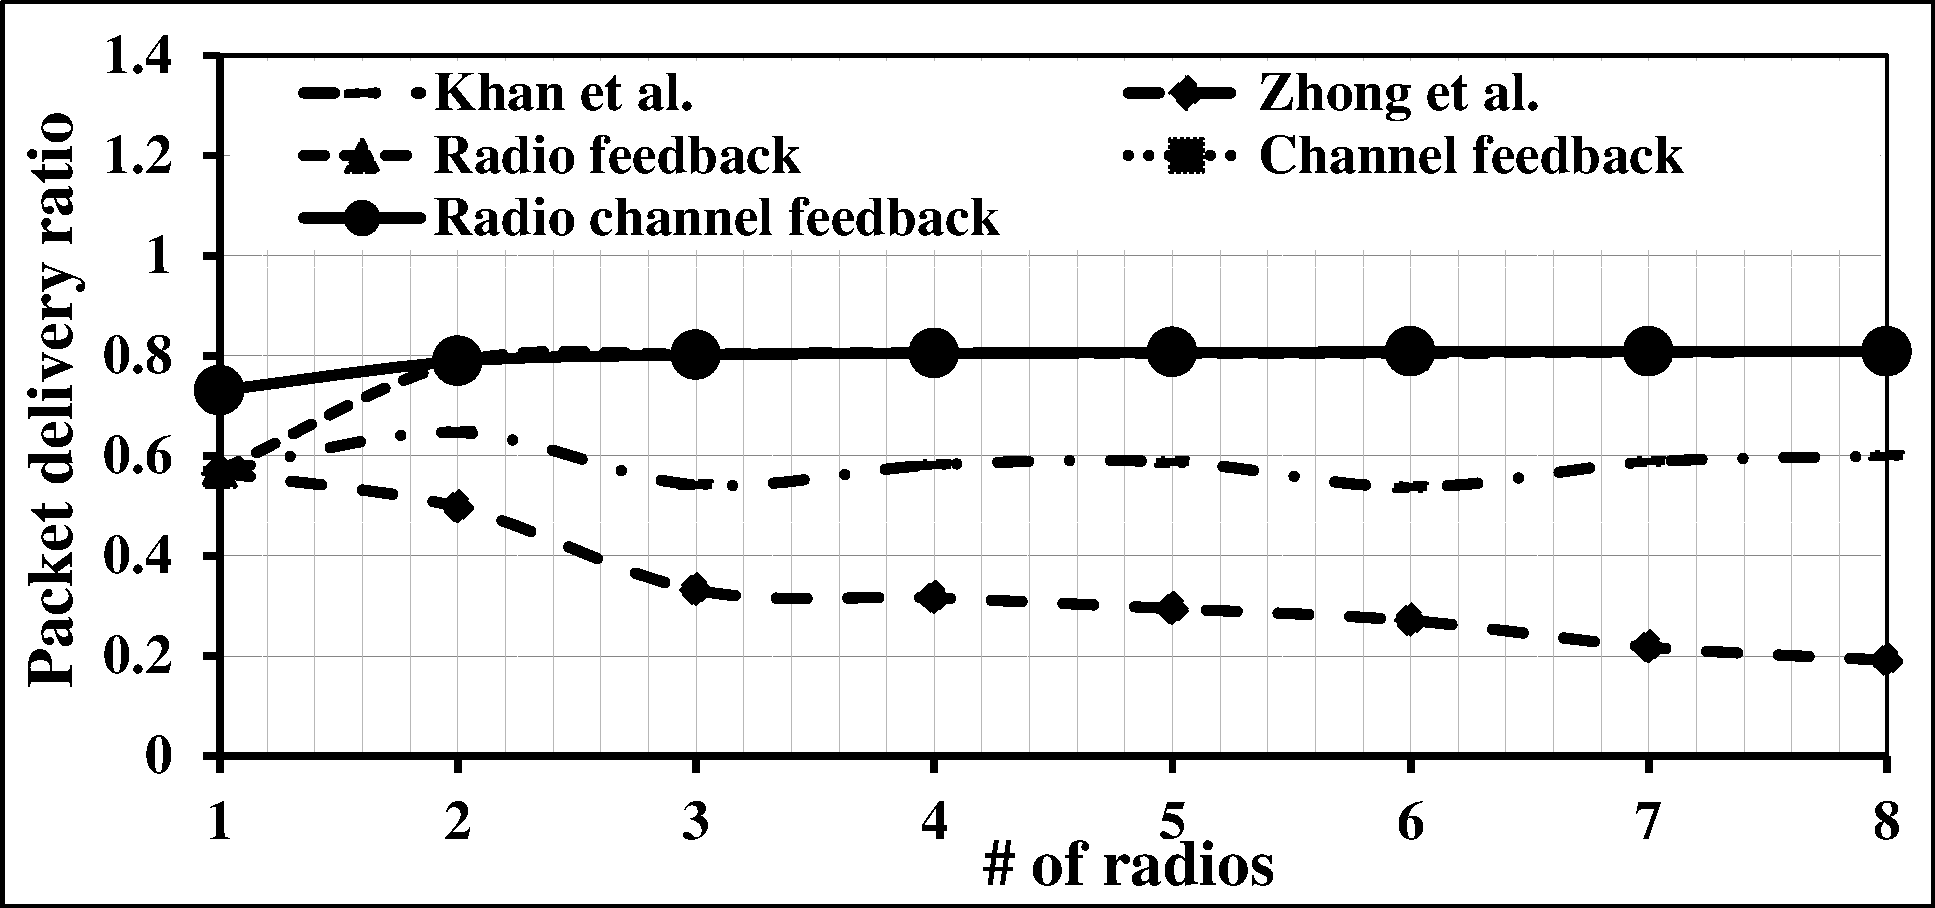
\includegraphics[width=\textwidth]{topology4/DeliveryRatio24d2}
        \caption{2Mbps application data rate}
        \label{fig:topology4PD2}
    \end{subfigure}
    ~\\
    \begin{subfigure}[t]{0.45\textwidth}
        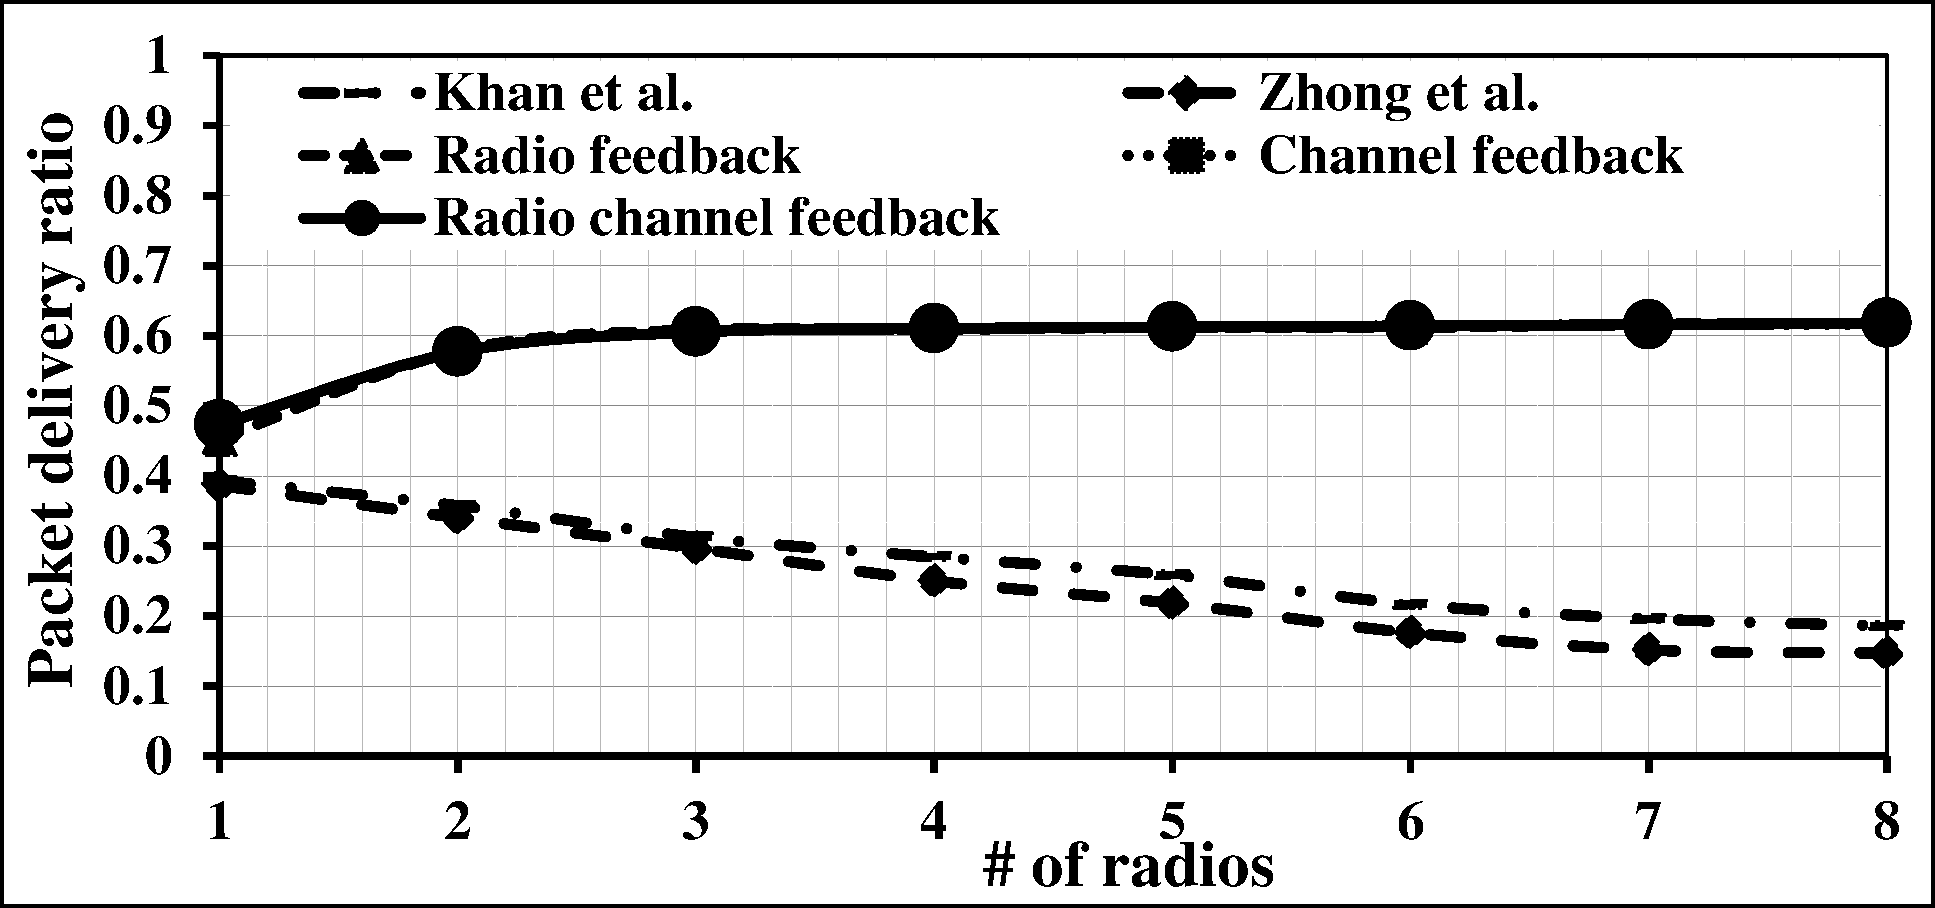
\includegraphics[width=\textwidth]{topology4/DeliveryRatio24d4}
        \caption{4Mbps application data rate}
        \label{fig:topology4PD3}
    \end{subfigure}
    ~
    \begin{subfigure}[t]{0.45\textwidth}
        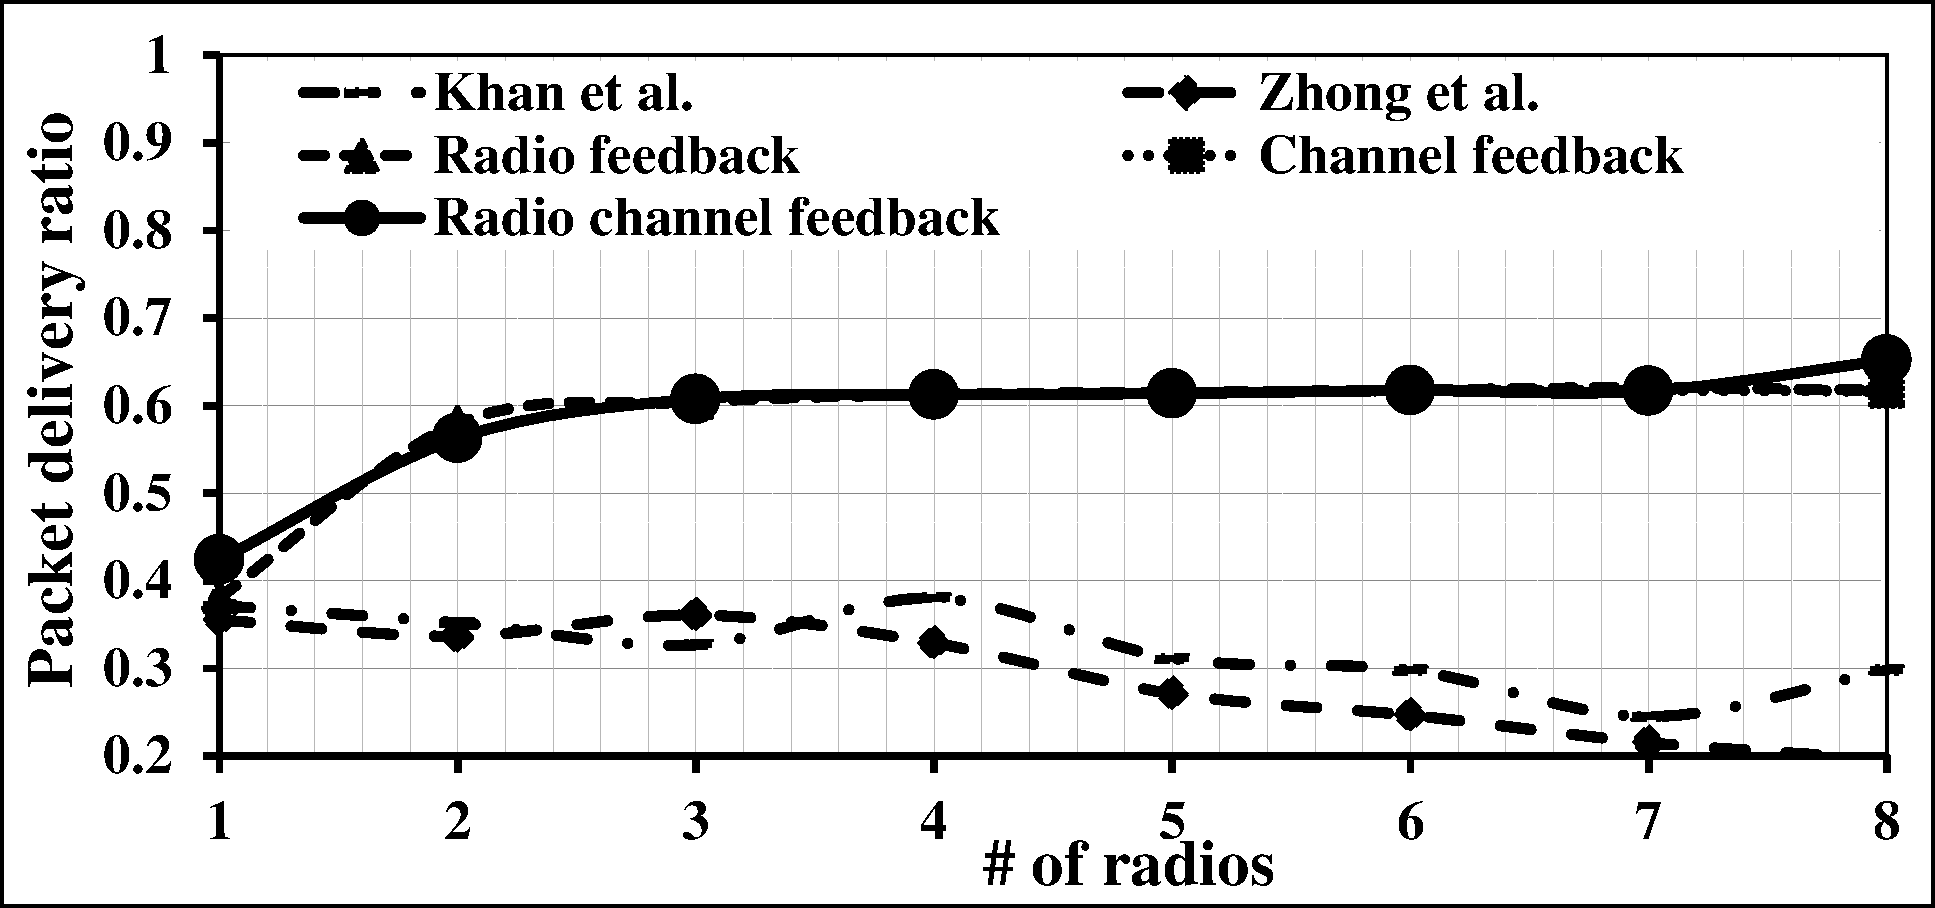
\includegraphics[width=\textwidth]{topology4/DeliveryRatio24d8}
        \caption{8Mbps application data rate}
        \label{fig:topology4PD4}
    \end{subfigure}
    ~\\
    \begin{subfigure}[t]{0.45\textwidth}
        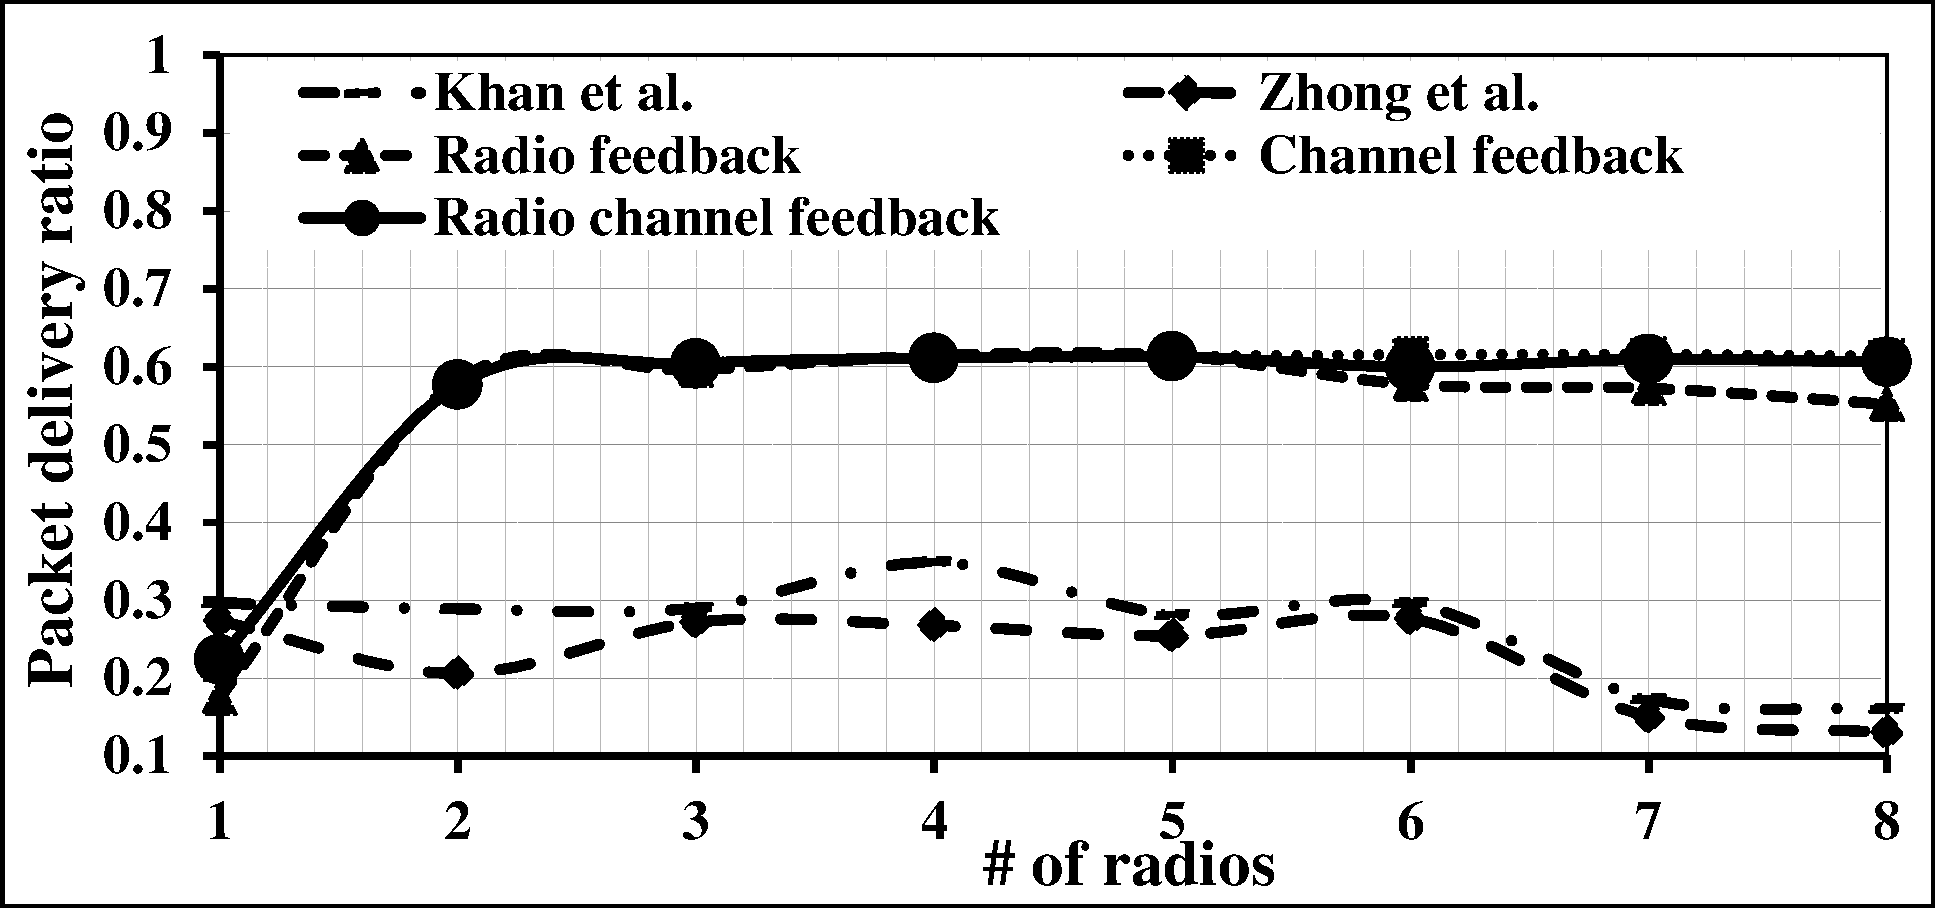
\includegraphics[width=\textwidth]{topology4/DeliveryRatio24d16}
        \caption{16Mbps application data rate}
        \label{fig:topology4PD5}
    \end{subfigure}
    ~
    \begin{subfigure}[t]{0.45\textwidth}
        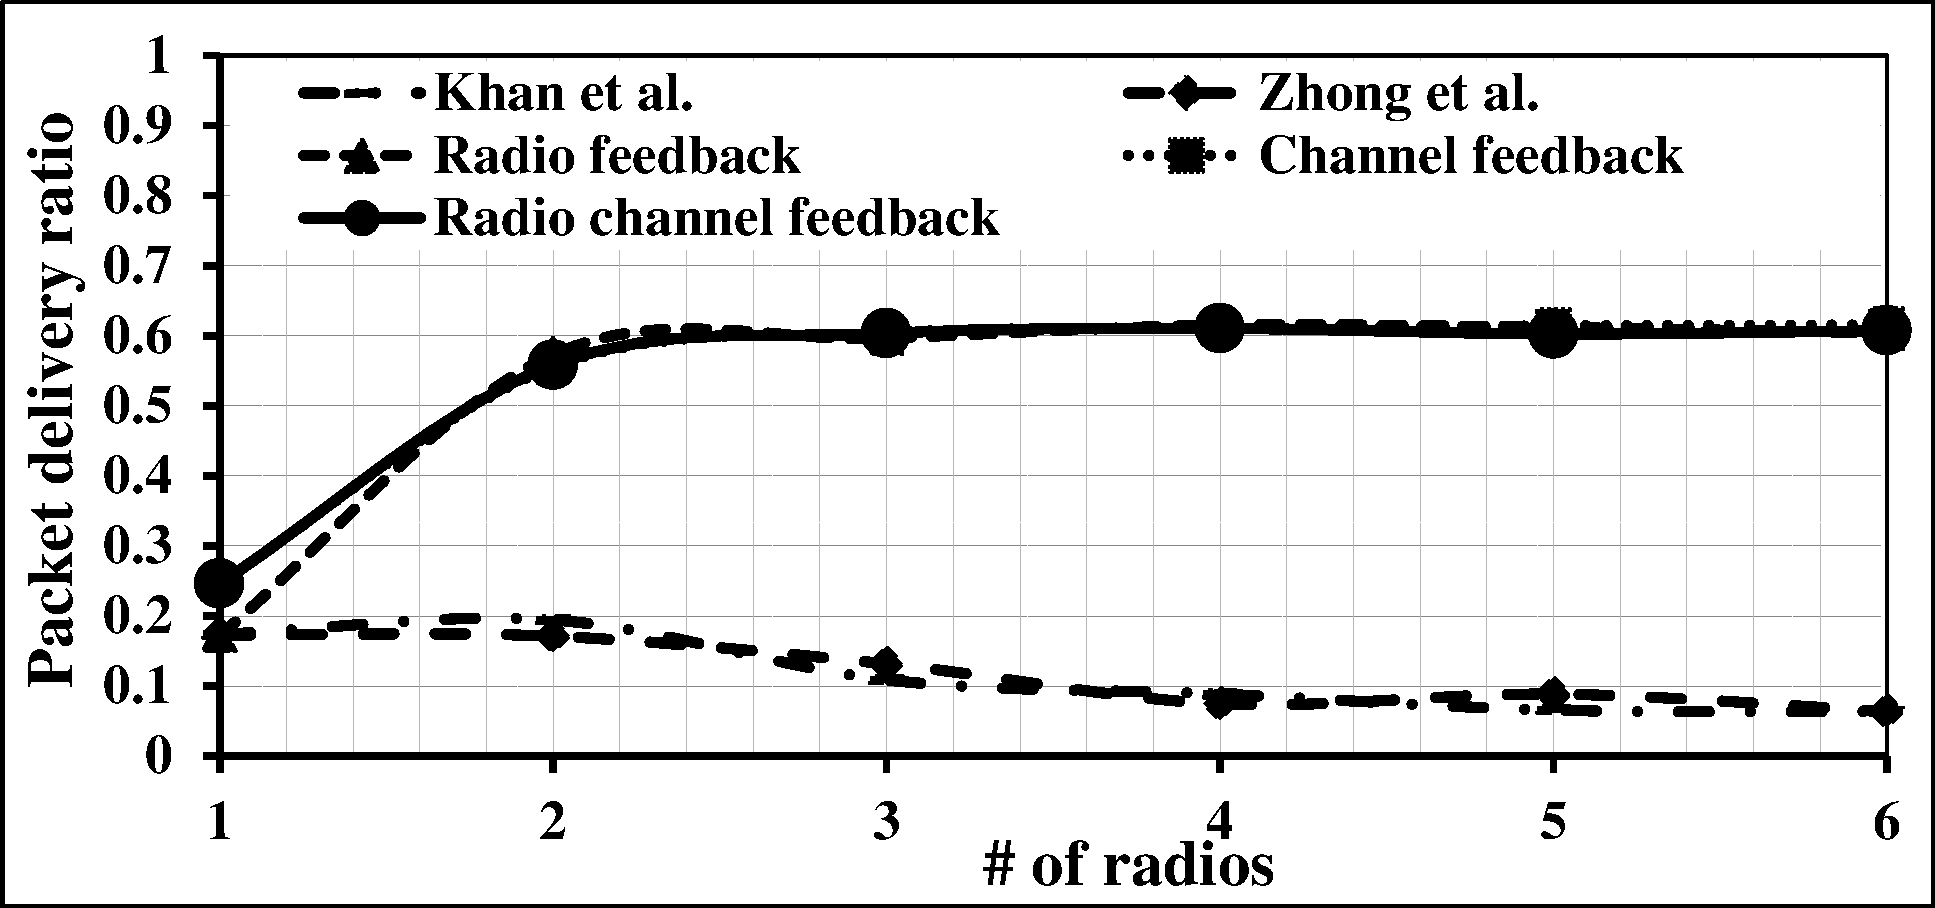
\includegraphics[width=\textwidth]{topology4/DeliveryRatio24d32}
        \caption{32Mbps application data rate}
        \label{fig:topology4PD6}
    \end{subfigure}
    \caption{Application layer packet delivery ratio with varying number of radios for various application data rates}
    \label{fig:topology4PD}
\end{figure*}


\begin{table}[!htb]
	\centering
    \caption{Performance improvement achieved using the radio feedback-based approach with respect to the approaches proposed by Khan et al.,~\cite{khan2015towards} and Zhong et al.,~\cite{zhong2014capacity}}
  \label{tab:topology4RadioImprovement}
  \renewcommand\multirowsetup{\centering}
    \begin{tabular}{|>{\centering} p{0.05\textwidth}|c|c|c|c|c|c|c|c|}
    \hline
    \multirow{2}{0.05\textwidth}{\newline \newline \newline Appli-\\cation data rate} & \multicolumn{2}{|p{0.08\textwidth}|}{\centering\% increase in throughput with respect to} & \multicolumn{2}{|p{0.08\textwidth}|}{\centering\% decrease in end-to-end delay with respect to} & \multicolumn{2}{|p{0.08\textwidth}|}{\centering\% decrease in packet drop ratio with respect to} & \multicolumn{2}{|p{0.08\textwidth}|}{\centering\% increase in application layer packet delivery ratio with respect to}\\
    \cline{2-9}
          & \multicolumn{1}{|p{0.025\textwidth}|}{\centering Khan et al.} & \multicolumn{1}{|p{0.025\textwidth}|}{\centering Zhong et al.} & \multicolumn{1}{|p{0.025\textwidth}|}{\centering Khan et al.} & \multicolumn{1}{|p{0.025\textwidth}|}{\centering Zhong et al.} & \multicolumn{1}{|p{0.03\textwidth}|}{\centering Khan et al.} & \multicolumn{1}{|p{0.025\textwidth}|}{\centering Zhong et al.} & \multicolumn{1}{|p{0.025\textwidth}|}{\centering Khan et al.} & \multicolumn{1}{|p{0.025\textwidth}|}{\centering Zhong et al.}\\
    \hline
    1Mbps & 55 & 14 & -9 & 48 & 57 & 57 & 12 & 12 \\\hline
    2Mbps & 64 & 33 & -10 & 50 & 52 & 54 & 24 & 27 \\\hline
    4Mbps & 66 & 44 & -16 & 45 & 40 & 41 & 52 & 52 \\\hline
    8Mbps & 63 & 46 & -17 & 32 & 26 & 26 & 42 & 43 \\\hline
    16Mbps & 62 & 48 & -16 & 24 & 18 & 18 & 40 & 46 \\\hline
    32Mbps & 63 & 42 & -13 & 28 & 13 & 12 & 69 & 73 \\\hline
    \end{tabular}%
\end{table}

\begin{table}[!htb]
	\centering
    \caption{Performance improvement achieved using the channel feedback-based approach with respect to the approaches proposed by Khan et al.,~\cite{khan2015towards} and Zhong et al.,~\cite{zhong2014capacity}}
  \label{tab:topology4ChannelImprovement}
  \renewcommand\multirowsetup{\centering}
    \begin{tabular}{|>{\centering} p{0.05\textwidth}|c|c|c|c|c|c|c|c|}
    \hline
    \multirow{2}{0.05\textwidth}{\newline \newline \newline Appli-\\cation data rate} & \multicolumn{2}{|p{0.08\textwidth}|}{\centering\% increase in throughput with respect to} & \multicolumn{2}{|p{0.08\textwidth}|}{\centering\% decrease in end-to-end delay with respect to} & \multicolumn{2}{|p{0.08\textwidth}|}{\centering\% decrease in packet drop ratio with respect to} & \multicolumn{2}{|p{0.08\textwidth}|}{\centering\% increase in application layer packet delivery ratio with respect to}\\
    \cline{2-9}
          & \multicolumn{1}{|p{0.025\textwidth}|}{\centering Khan et al.} & \multicolumn{1}{|p{0.025\textwidth}|}{\centering Zhong et al.} & \multicolumn{1}{|p{0.025\textwidth}|}{\centering Khan et al.} & \multicolumn{1}{|p{0.025\textwidth}|}{\centering Zhong et al.} & \multicolumn{1}{|p{0.03\textwidth}|}{\centering Khan et al.} & \multicolumn{1}{|p{0.025\textwidth}|}{\centering Zhong et al.} & \multicolumn{1}{|p{0.025\textwidth}|}{\centering Khan et al.} & \multicolumn{1}{|p{0.025\textwidth}|}{\centering Zhong et al.}\\
    \hline
    1Mbps & 55 & 15 & -8 & 49 & 58 & 58 & 12 & 41 \\\hline 
    2Mbps & 63 & 31 & -15 & 48 & 51 & 51 & 27 & 55 \\\hline 
    4Mbps & 66 & 44 & -11 & 42 & 40 & 38 & 52 & 52 \\\hline 
    8Mbps & 64 & 49 & -16 & 31 & 30 & 30 & 44 & 48\\\hline 
    16Mbps & 68 & 55 & -13 & 25 & 21 & 20 & 45 & 47 \\\hline 
    32Mbps & 64 & 44 & -16 & 23 & 15 & 15 & 73 & 68 \\\hline 
    \end{tabular}%
\end{table}

\begin{table}[!htb]
	\centering
    \caption{Performance improvement achieved using the radio channel feedback-based approach with respect to the approaches proposed by Khan et al.,~\cite{khan2015towards} and Zhong et al.,~\cite{zhong2014capacity}}
  \label{tab:topology4RadioChannelImprovement}
  \renewcommand\multirowsetup{\centering}
    \begin{tabular}{|>{\centering} p{0.05\textwidth}|c|c|c|c|c|c|c|c|}
    \hline
    \multirow{2}{0.05\textwidth}{\newline \newline \newline Appli-\\cation data rate} & \multicolumn{2}{|p{0.08\textwidth}|}{\centering\% increase in throughput with respect to} & \multicolumn{2}{|p{0.08\textwidth}|}{\centering\% decrease in end-to-end delay with respect to} & \multicolumn{2}{|p{0.08\textwidth}|}{\centering\% decrease in packet drop ratio with respect to} & \multicolumn{2}{|p{0.08\textwidth}|}{\centering\% increase in application layer packet delivery ratio with respect to}\\
    \cline{2-9}
          & \multicolumn{1}{|p{0.025\textwidth}|}{\centering Khan et al.} & \multicolumn{1}{|p{0.025\textwidth}|}{\centering Zhong et al.} & \multicolumn{1}{|p{0.025\textwidth}|}{\centering Khan et al.} & \multicolumn{1}{|p{0.025\textwidth}|}{\centering Zhong et al.} & \multicolumn{1}{|p{0.03\textwidth}|}{\centering Khan et al.} & \multicolumn{1}{|p{0.025\textwidth}|}{\centering Zhong et al.} & \multicolumn{1}{|p{0.025\textwidth}|}{\centering Khan et al.} & \multicolumn{1}{|p{0.025\textwidth}|}{\centering Zhong et al.}\\
    \hline 
    1Mbps & 55 & 15 & -18 & 49 & 58 & 58 & 42 & 42 \\\hline 
    2Mbps & 63 & 31 & -15 & 49 & 51 & 51 & 58 & 58 \\\hline 
    4Mbps & 66 & 44 & -17 & 42 & 40 & 41 & 57 & 57 \\\hline 
    8Mbps & 63 & 49 & -17 & 31 & 29 & 30 & 49 & 50 \\\hline 
    16Mbps & 68 & 55 & -14 & 27 & 21 & 20 & 53 & 52 \\\hline 
    32Mbps & 64 & 43 & -13 & 23 & 15 & 15 & 73 & 73 \\\hline 
    \end{tabular}%
    \vspace{-0.625cm}
\end{table}


\iffalse
% Table generated by Excel2LaTeX from sheet 'Sheet1'
\begin{table*}[!htbp]
  \centering
  \caption{Percentage improvement achieved using the feedback-based approach with respect to the approaches proposed by Khan et al.,~\cite{khan2015towards} and Zhong et al.,~\cite{zhong2014capacity}}
  \label{tab:topology4Improvement}
    \begin{tabular}{ccccccc}
    \toprule
    \multirow{2}[0]{*}{Application data rate} & \multicolumn{2}{p{0.2\textwidth}}{\% increase in total network througput w.r.t} & \multicolumn{2}{p{0.2\textwidth}}{\% decrease in per packet end-to-end delay w.r.t} & \multicolumn{2}{p{0.2\textwidth}}{\% decrease in packet drop ratio w.r.t} \\
          & \multicolumn{1}{l}{Khan et al.} & \multicolumn{1}{l}{Zhong et al.} & \multicolumn{1}{l}{Khan et al.} & \multicolumn{1}{l}{Zhong et al.} & \multicolumn{1}{l}{Khan et al.} & \multicolumn{1}{l}{Zhong et al.} \\
    \midrule
    1Mbps & 55.862076 & 16.77937765 & -15.155181 & 50.73693391 & 59.865701 & 59.8842253 \\
    2Mbps & 64.74406156 & 33.88792815 & -17.680018 & 51.43200614 & 53.816642 & 53.5899378 \\
    4Mbps & 67.37679147 & 45.85754947 & -30.950717 & 45.37420031 & 41.190572 & 41.8005298 \\
    8Mbps & 65.2701612 & 49.89498939 & -36.956627 & 33.28484049 & 29.774189 & 29.9230113 \\
    16Mbps & 68.48584166 & 55.17376536 & -24.008348 & 28.92168644 & 21.287883 & 20.6884369 \\
    32Mbps & 65.62299103 & 45.56263021 & -13.078491 & 28.3215896 & 15.364822 & 14.5973083 \\
    \bottomrule
    \end{tabular}%
\end{table*}%
\fi


\subsection{Simulation Findings}

Though we have performed discrete event simulations for various network topologies varying the number of secondary users from 12 to 40 with a granularity of 4, in this paper, due to space limitation, we have presented the simulation results for only one topology with 24 secondary users. Our proposed approach for CMRNs obtains similar results in case of other seven network topologies as well. Over all these topologies, our feedback-based approach improves total network throughput 51\% and decrease packet drop ratio up to 35\% on an average against that of existing approaches. Among three variants of our proposed approach, radio channel feedback approach marginally better over other variants.

%\section{Future Work}
\vspace{-0.25cm}
\section{Conclusion}
\vspace{-0.25cm}
Cognitive radio networks suffer noteworthy throughput degradation with the introduction of multi-radio usage. We propose a feedback-based multi-radio exploitation approach for CRNs in this paper to overcome this throughput degradation. We implement the proposed approach in ns-3 to measure various performance metrics such as throughput, delay, packet delivery, and drop ratio over numerous network settings. Simulation results reveal that our proposed approach can significantly increase total network throughput and decrease packet drop ratio compared to other existing techniques. Furthermore, the feedback-based approach can be used to find the number of radios needed to experience a delicate tradeoff between network throughput and delay for applications maintaining different data rates. In future, we plan to formulate analytical models of our proposed approach and implement the approach in real testbed.

%However, further study is required to mathematical model these performance metrics under such feedback-based multi-radio exploitation. We leave this for future work.
\iffalse
\section*{Acknowledgment}
This work has been conducted at and partially supported by Bangladesh University of Engineering and Technology (BUET), Dhaka, Bangladesh.
\fi

\vspace{-0.5cm}
\bibliographystyle{unsrt}
{\tiny
\bibliography{SystemModel}}

\end{document}
